\documentclass[journal]{IEEEtran}
\usepackage[a5paper, margin=10mm]{geometry}
%\usepackage{lmodern} % Ensure lmodern is loaded for pdflatex
\usepackage{tfrupee} % Include tfrupee package

\setlength{\headheight}{1cm}
\setlength{\headsep}{0mm}

\usepackage{gvv-book}
\usepackage{gvv}
\usetikzlibrary{patterns}
\lstset{aboveskip=12pt}
\usepackage[center]{caption}
\raggedbottom

\hypersetup{
    colorlinks=true,
    urlcolor=black
}
\usepackage{amsfonts}
\makeindex

\begin{document}
\bibliographystyle{IEEEtran}
\onecolumn

\title{
    \begin{center}
        Math for EE
        \\
        \rule{0.4\columnwidth}{0.4pt}
    \end{center}
}
\author{
    \vspace{11cm}
    \begin{center}
        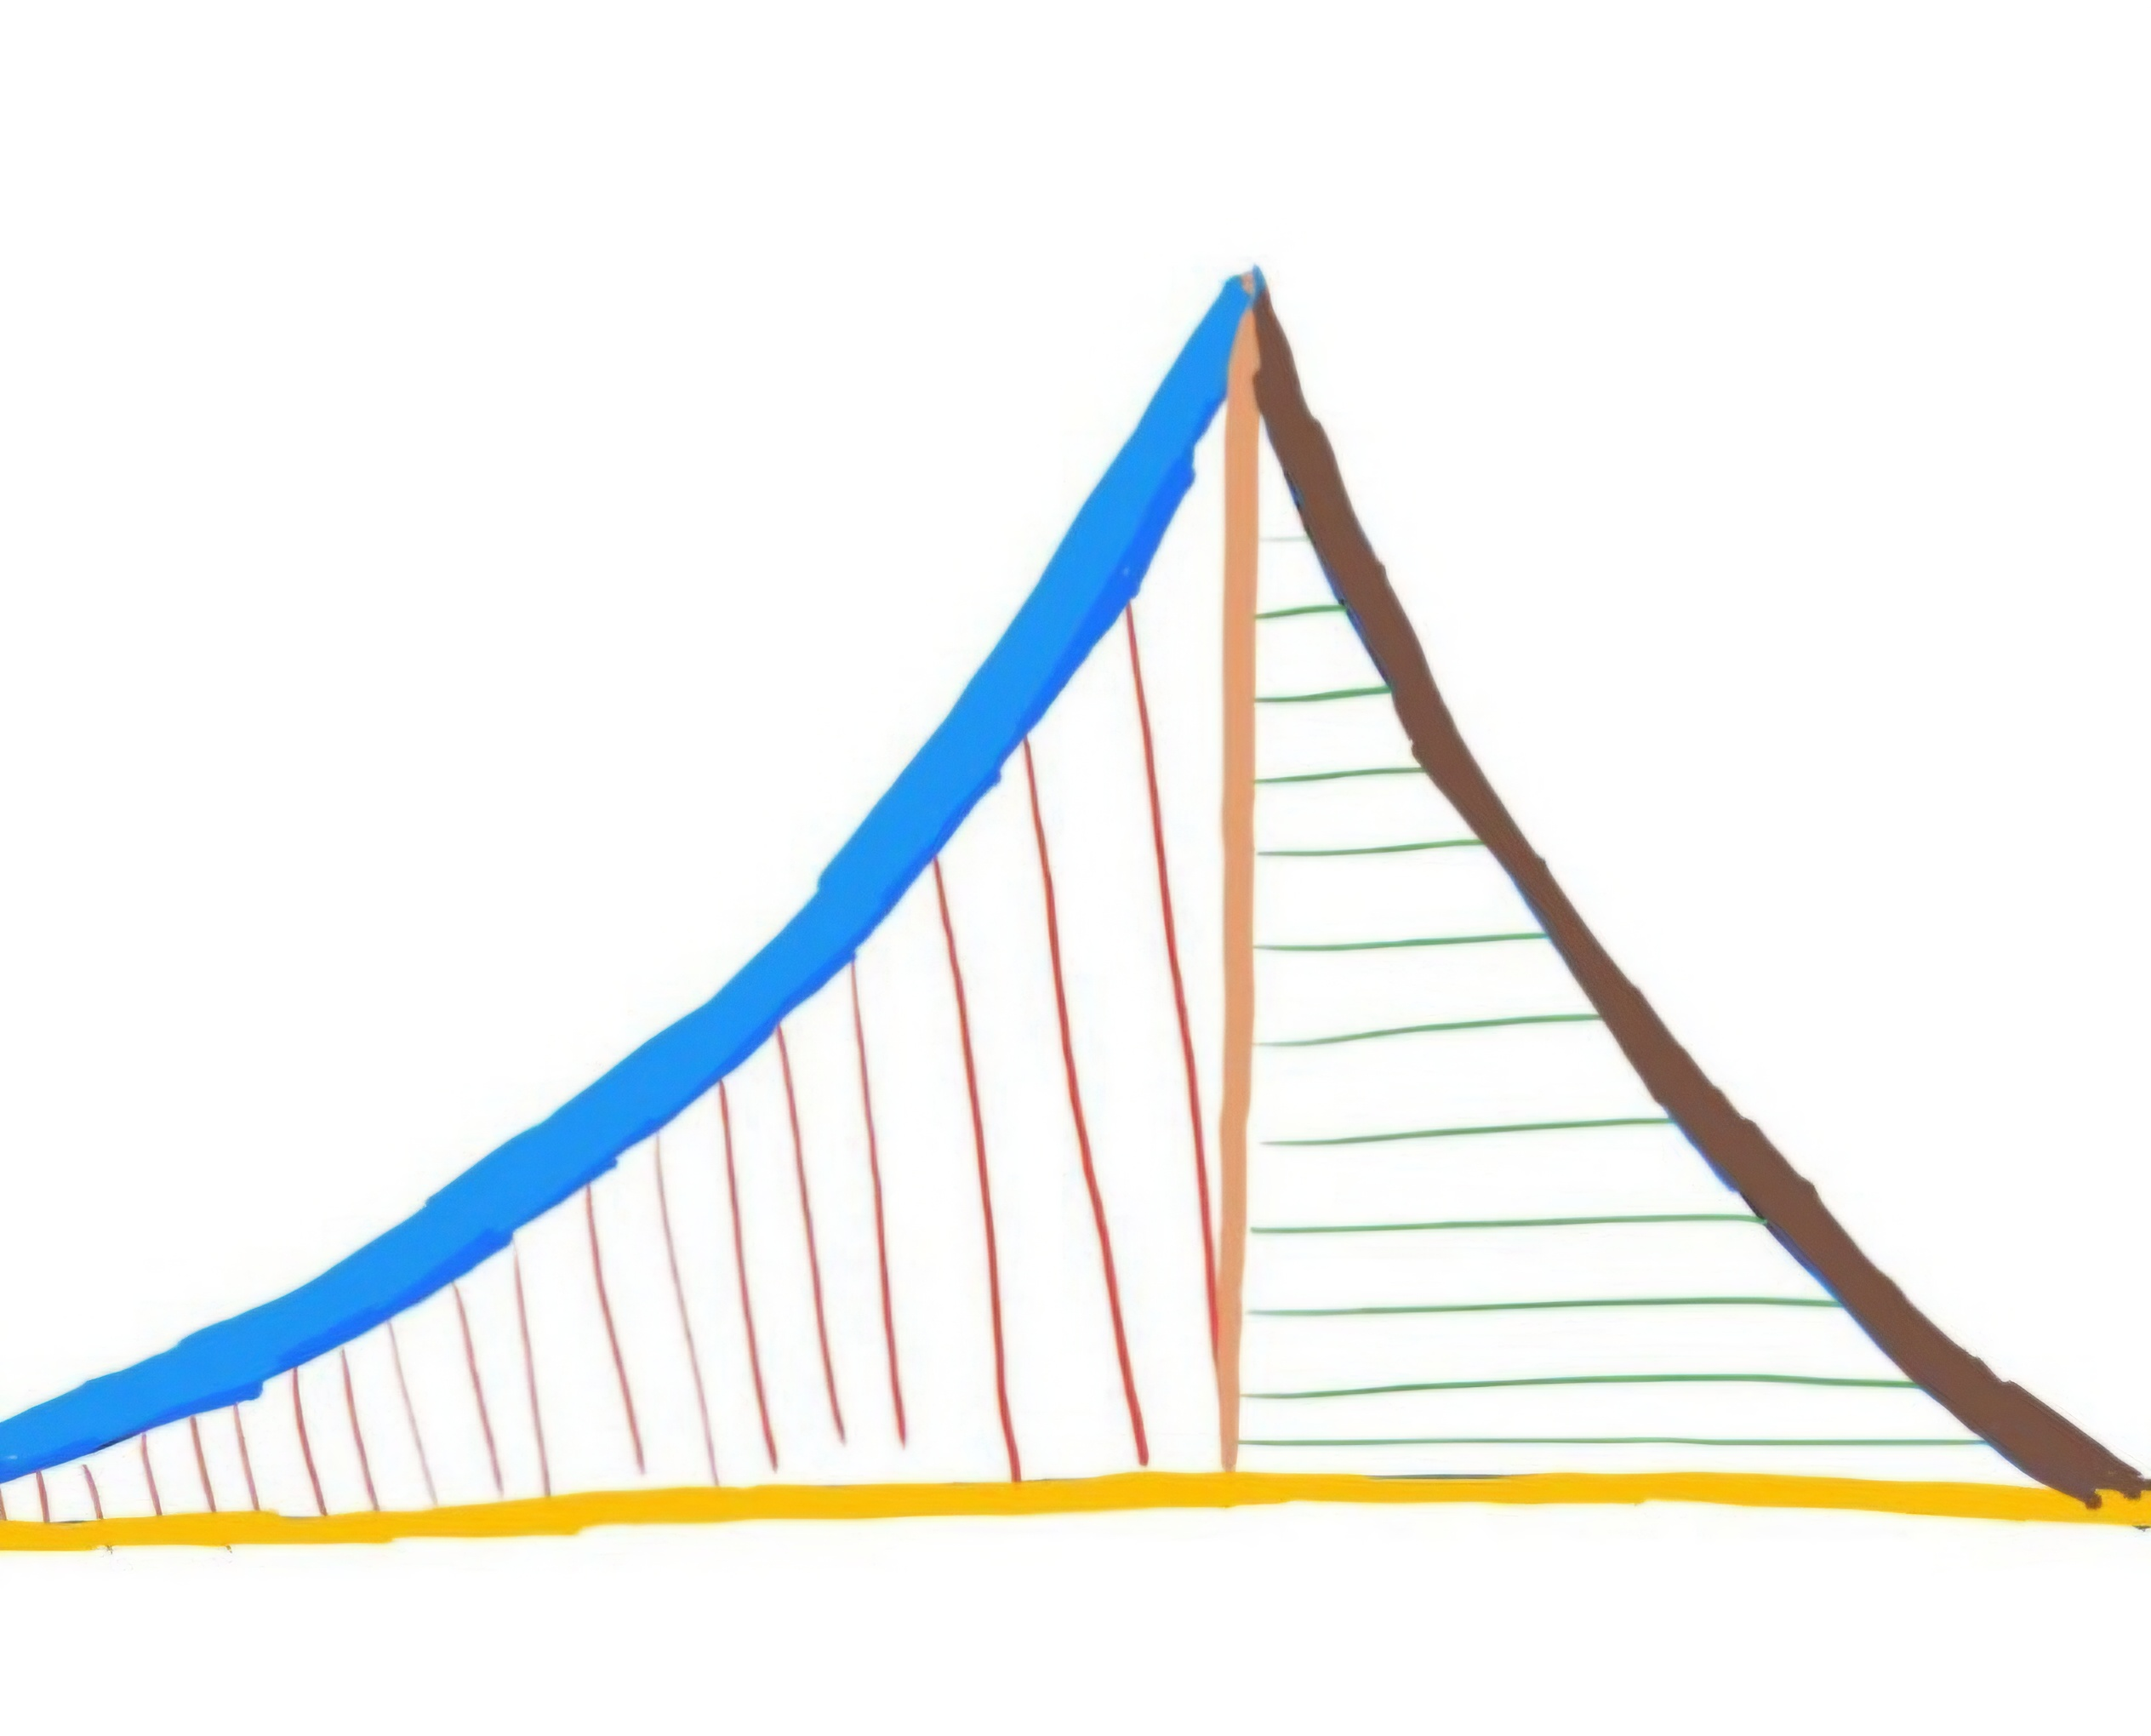
\includegraphics[width=0.2\columnwidth]{figs/logo.jpg}
        \\
        {\huge G. V. V. Sharma}
    \end{center}
}
\maketitle

\newpage
\section*{About this Book}

This book introduces matrices through high school coordinate geometry.
This approach makes it easier for beginners to learn Python for scientific
computing. All problems in the book are from NCERT mathematics textbooks
from Class 9--12. Exercises are from CBSE board exam papers.

The content is sufficient for industry jobs and covers nearly all matrix
prerequisites for machine learning. There is no copyright, so readers are
free to print and share.
License: https://creativecommons.org/licenses/by-sa/3.0/
\\
and
\\
https://www.gnu.org/licenses/fdl-1.3.en.html
\\
First manual appeared in January 2018
\\
First edition published on July 10, 2024
\\
In this edition, some incorrect solutions were removed. All figures
redrawn. More problems added.

\newpage
\onecolumn
\begin{center}
{\Large\bfseries CBSE 2026 10th class maths set A solutions}
\end{center}
\vspace{0.4em}
\begin{list}{}{\setlength{\leftmargin}{1.15cm}\setlength{\labelwidth}{1.0cm}\setlength{\labelsep}{0.15cm}\setlength{\itemindent}{0pt}\setlength{\listparindent}{0pt}\setlength{\parsep}{0pt}\setlength{\topsep}{0pt}}\setlist[enumerate]{leftmargin=0.7cm}
\item[5.1.1] The value of $k$ for which the equation
\[
kx^2 - 6x - 4 = 0
\]
has real and equal roots is:

\begin{enumerate}
    \item[(A)] \(\frac{9}{4}\)
    \item[(B)] \(-4\)
    \item[(C)] \(-\frac{9}{4}\)
    \item[(D)] \(-2\)
\end{enumerate}

\vspace{0.7em}\par\noindent\textbf{Solution:}

For a quadratic equation $ax^2 + bx + c = 0$, the roots are real and equal when 
\[
b^2 - 4ac = 0.
\]
Here, $a = k$, $b = -6$, and $c = -4$. Therefore,
\[
(-6)^2 - 4(k)(-4) = 0,
\]
\[
36 + 16k = 0,
\]
so
\[
\boxed{k = -\frac{9}{4}}.
\]

The correct answer is \textbf{(C)}.
The following code generates Figure~\ref{fig:q1-graph}.

\begin{lstlisting}[frame=single, basicstyle=\rmfamily, escapeinside={(*@}{@*)}]
(*@\makebox[\dimexpr\linewidth-2\fboxsep-2\fboxrule\relax][c]{codes/5.1.1.py}@*)
\end{lstlisting}
\begin{figure}[H]
    \centering
    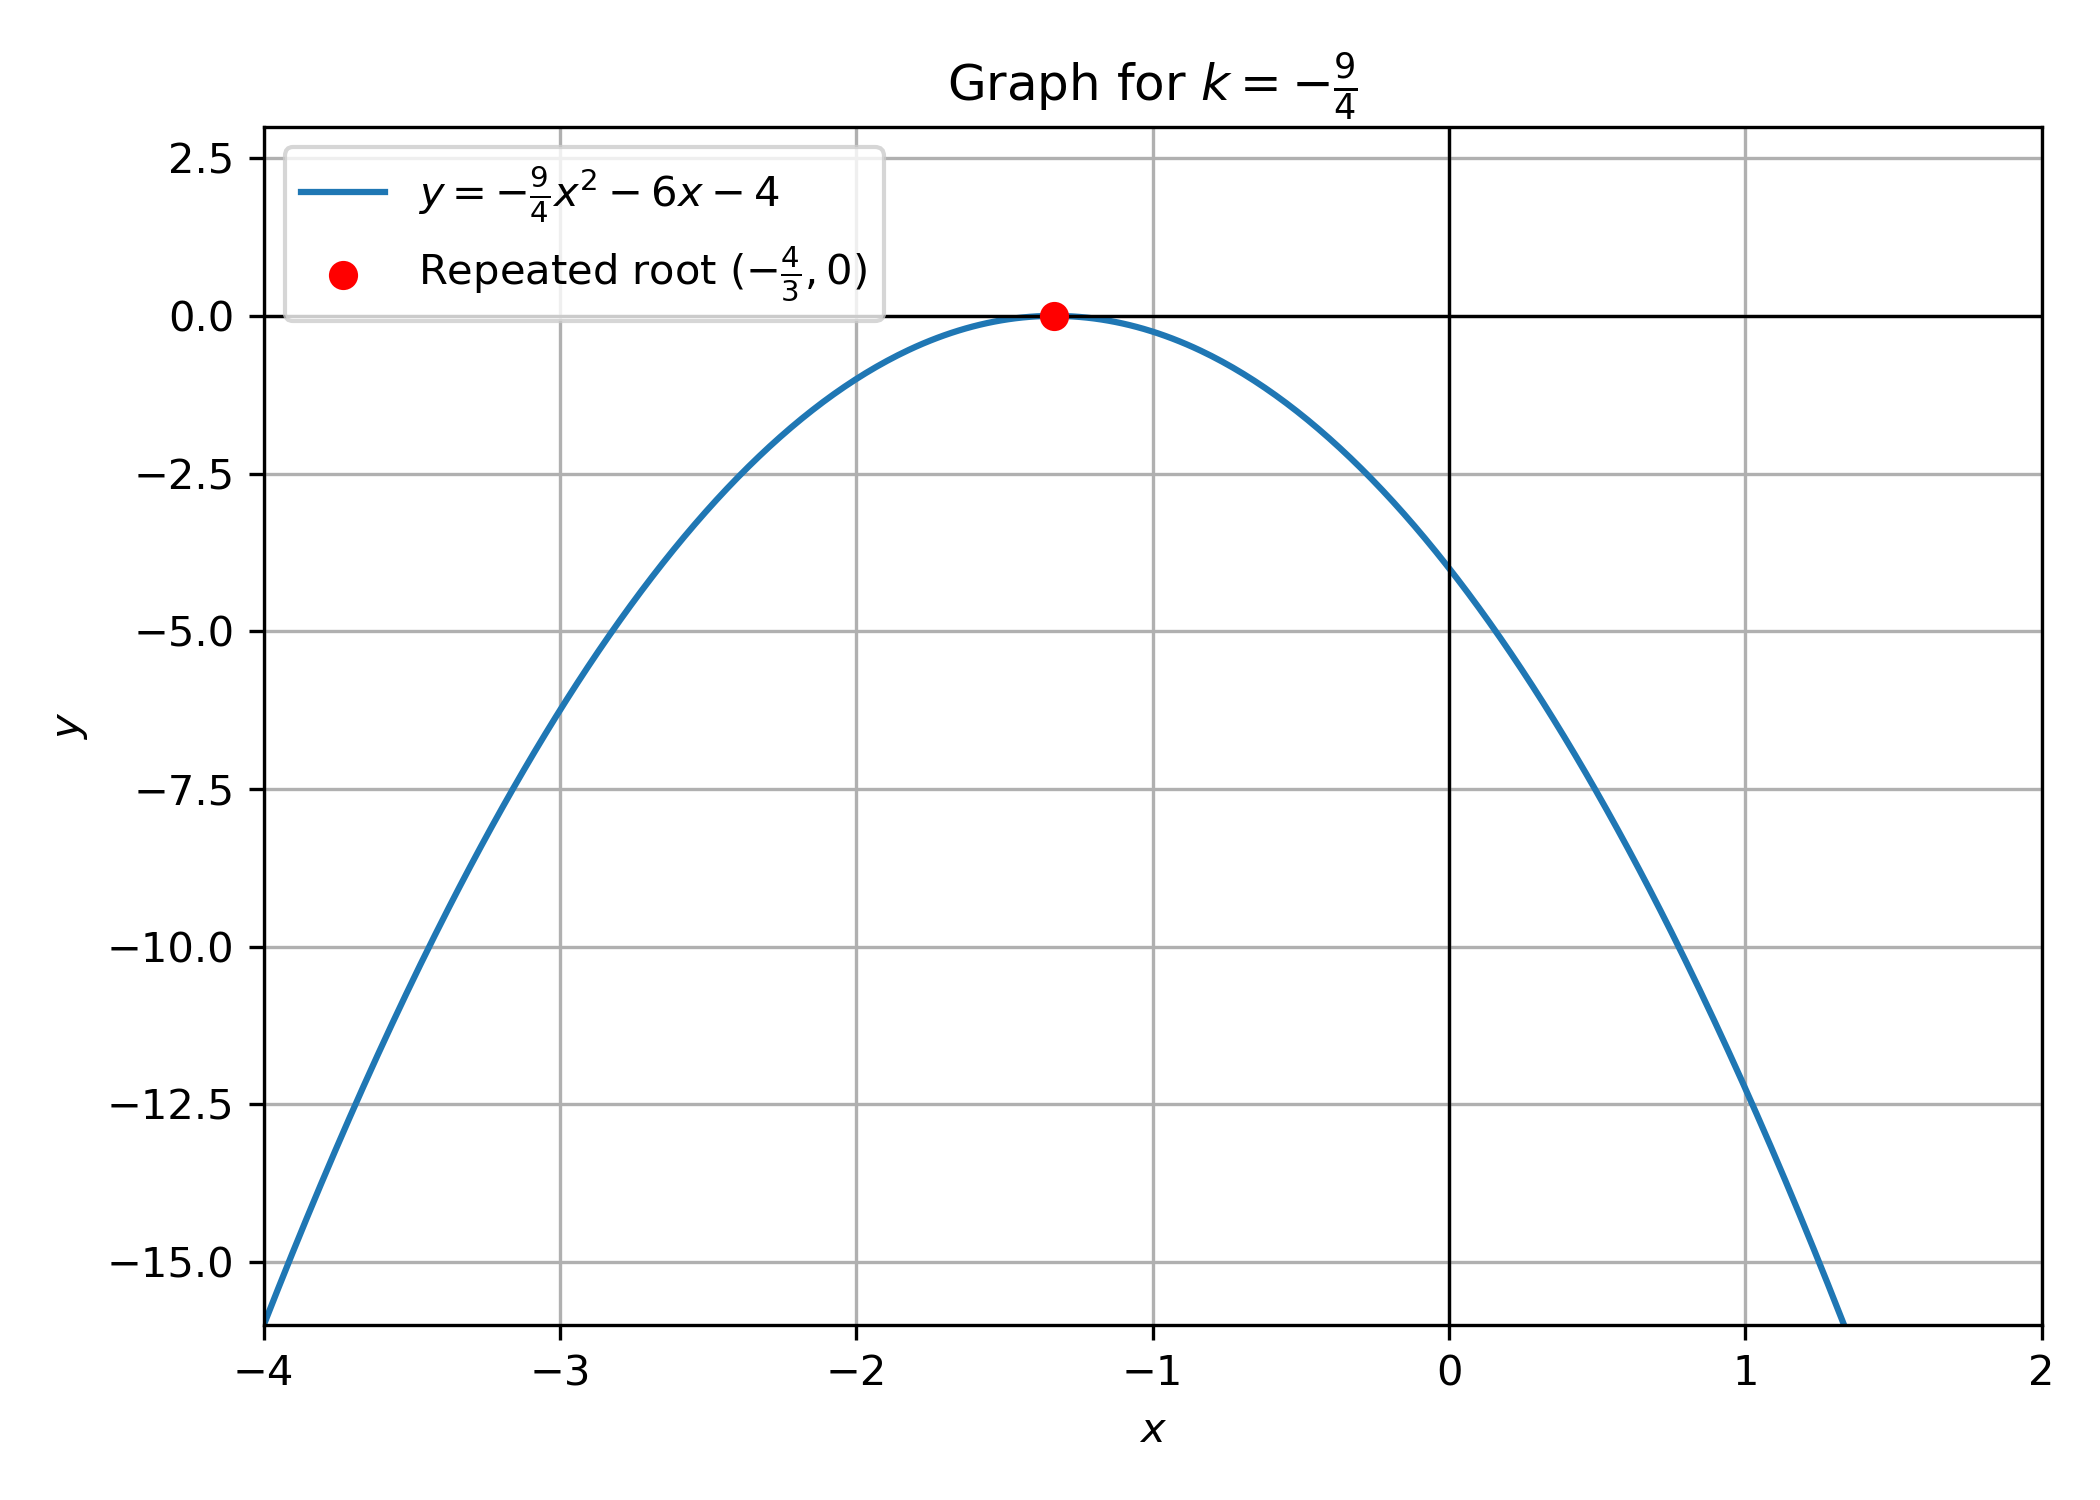
\includegraphics[width=0.60\linewidth]{figs/5.1.1.png}
    \caption{Graph of $y = -\frac{9}{4}x^2 - 6x - 4$, tangent to the $x$-axis at $x = -\frac{4}{3}$.}
    \label{fig:q1-graph}
\end{figure}


\end{list}
\vspace{1.2em}
\begin{list}{}{\setlength{\leftmargin}{1.15cm}\setlength{\labelwidth}{1.0cm}\setlength{\labelsep}{0.15cm}\setlength{\itemindent}{0pt}\setlength{\listparindent}{0pt}\setlength{\parsep}{0pt}\setlength{\topsep}{0pt}}\setlist[enumerate]{leftmargin=0.7cm}
\item[5.1.2] The line segment joining the points $P(-4,-2)$ and $Q(10,4)$ is divided by the $y$-axis in the ratio:

\begin{enumerate}
    \item[(A)] $2:5$
    \item[(B)] $1:2$
    \item[(C)] $2:1$
    \item[(D)] $5:2$
\end{enumerate}

\vspace{0.7em}\par\noindent\textbf{Solution:}

Let $R$ be the point where the segment meets the $y$-axis, and let $PR:RQ=m:n$. Since $R$ lies on the $y$-axis, its $x$-coordinate is zero. By the section formula,
\[
0 = \frac{10m - 4n}{m+n}.
\]
Thus,
\[
10m - 4n = 0 \quad\Longrightarrow\quad 5m = 2n,
\]
so
\[
PR:RQ = m:n = 2:5.
\]
The correct answer is \textbf{(A)}. The coordinates of the intersection point are
\[
R = \left(0,-\frac{2}{7}\right).
\]

The following code generates Figure~\ref{fig:q2-graph}.
\begin{lstlisting}[frame=single, basicstyle=\rmfamily, escapeinside={(*@}{@*)}]
(*@\makebox[\dimexpr\linewidth-2\fboxsep-2\fboxrule\relax][c]{codes/5.1.2.py}@*)
\end{lstlisting}
\begin{figure}[H]
    \centering
    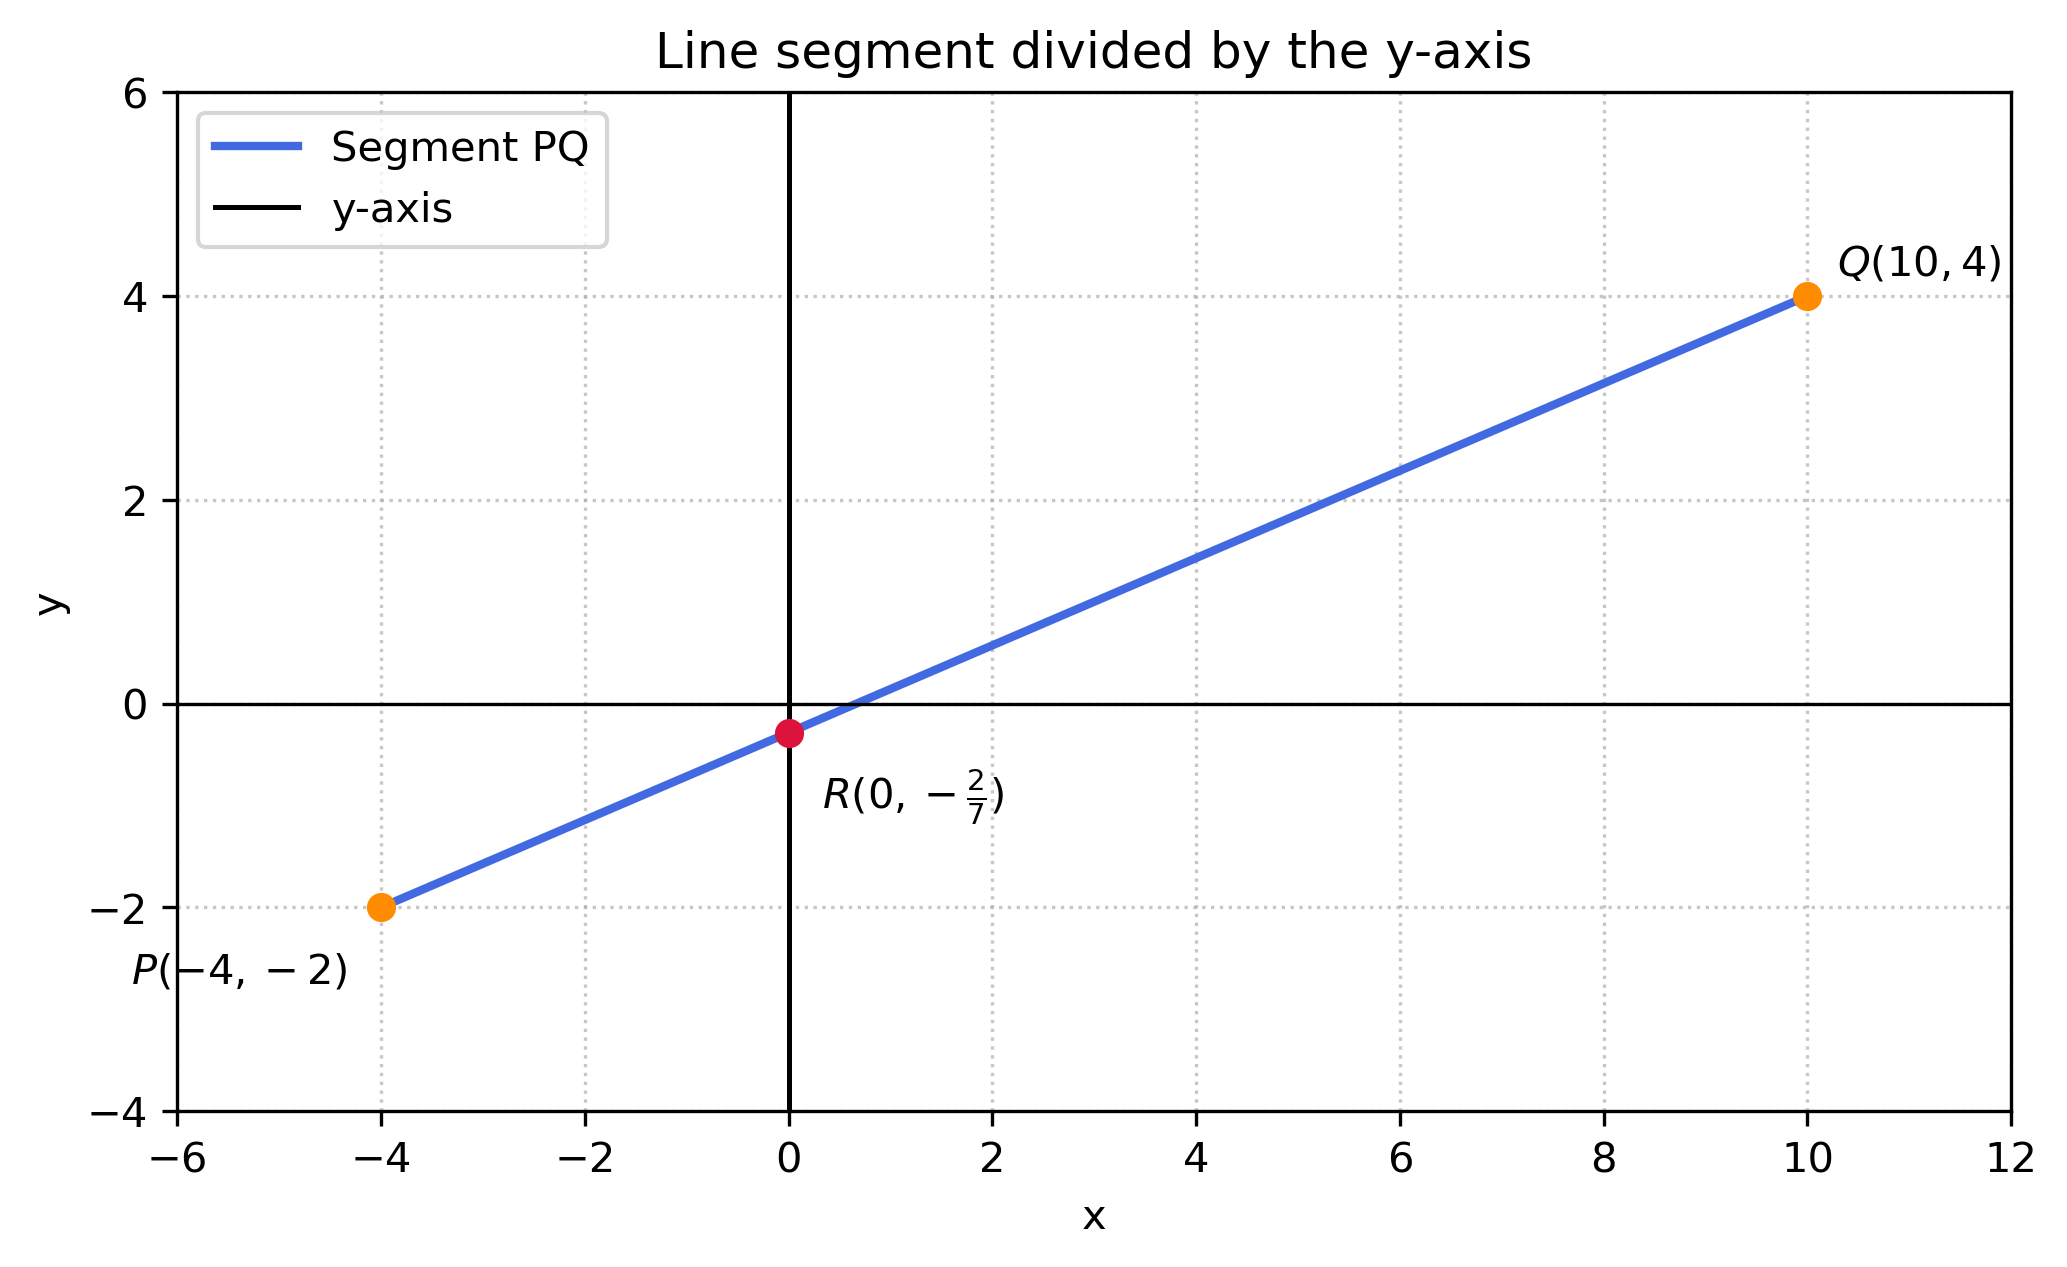
\includegraphics[width=0.60\linewidth]{figs/5.1.2.png}
    \caption{The segment $PQ$ and its intersection $R$ with the $y$-axis.}
    \label{fig:q2-graph}
\end{figure}
\end{list}
\vspace{1.2em}
\begin{list}{}{\setlength{\leftmargin}{1.15cm}\setlength{\labelwidth}{1.0cm}\setlength{\labelsep}{0.15cm}\setlength{\itemindent}{0pt}\setlength{\listparindent}{0pt}\setlength{\parsep}{0pt}\setlength{\topsep}{0pt}}\setlist[enumerate]{leftmargin=0.7cm}
\item[5.1.4] In the given figure, $PQ$ is tangent to the circle with centre $O$. $S$ is a point on the circle such that $\angle SQT = 55^\circ$. The measure of $\angle QPS$ is:

\begin{enumerate}
    \item[(A)] $55^\circ$
    \item[(B)] $20^\circ$
    \item[(C)] $35^\circ$
    \item[(D)] $70^\circ$
\end{enumerate}

\vspace{0.7em}\par\noindent\textbf{Solution:}

The radius $OQ$ is perpendicular to the tangent $QT$. Hence,
\[
\angle OQS = 90^\circ - 55^\circ = 35^\circ.
\]
Since $OQ = OS$, triangle $OQS$ is isosceles, so $\angle QSO = 35^\circ$. The points $P$, $O$, and $S$ are collinear, giving $\angle QSP = 35^\circ$. Also, $QP$ and $QT$ are opposite rays, so
\[
\angle PQS = 180^\circ - 55^\circ = 125^\circ.
\]
Therefore, in triangle $PQS$,
\[
\angle QPS = 180^\circ - 125^\circ - 35^\circ = 20^\circ.
\]
The correct answer is \textbf{(B)}.

The following code generates Figure~\ref{fig:q4-graph}.
\begin{lstlisting}[frame=single, basicstyle=\rmfamily, escapeinside={(*@}{@*)}]
(*@\makebox[\dimexpr\linewidth-2\fboxsep-2\fboxrule\relax][c]{codes/5.1.4.py}@*)
\end{lstlisting}
\begin{figure}[H]
    \centering
    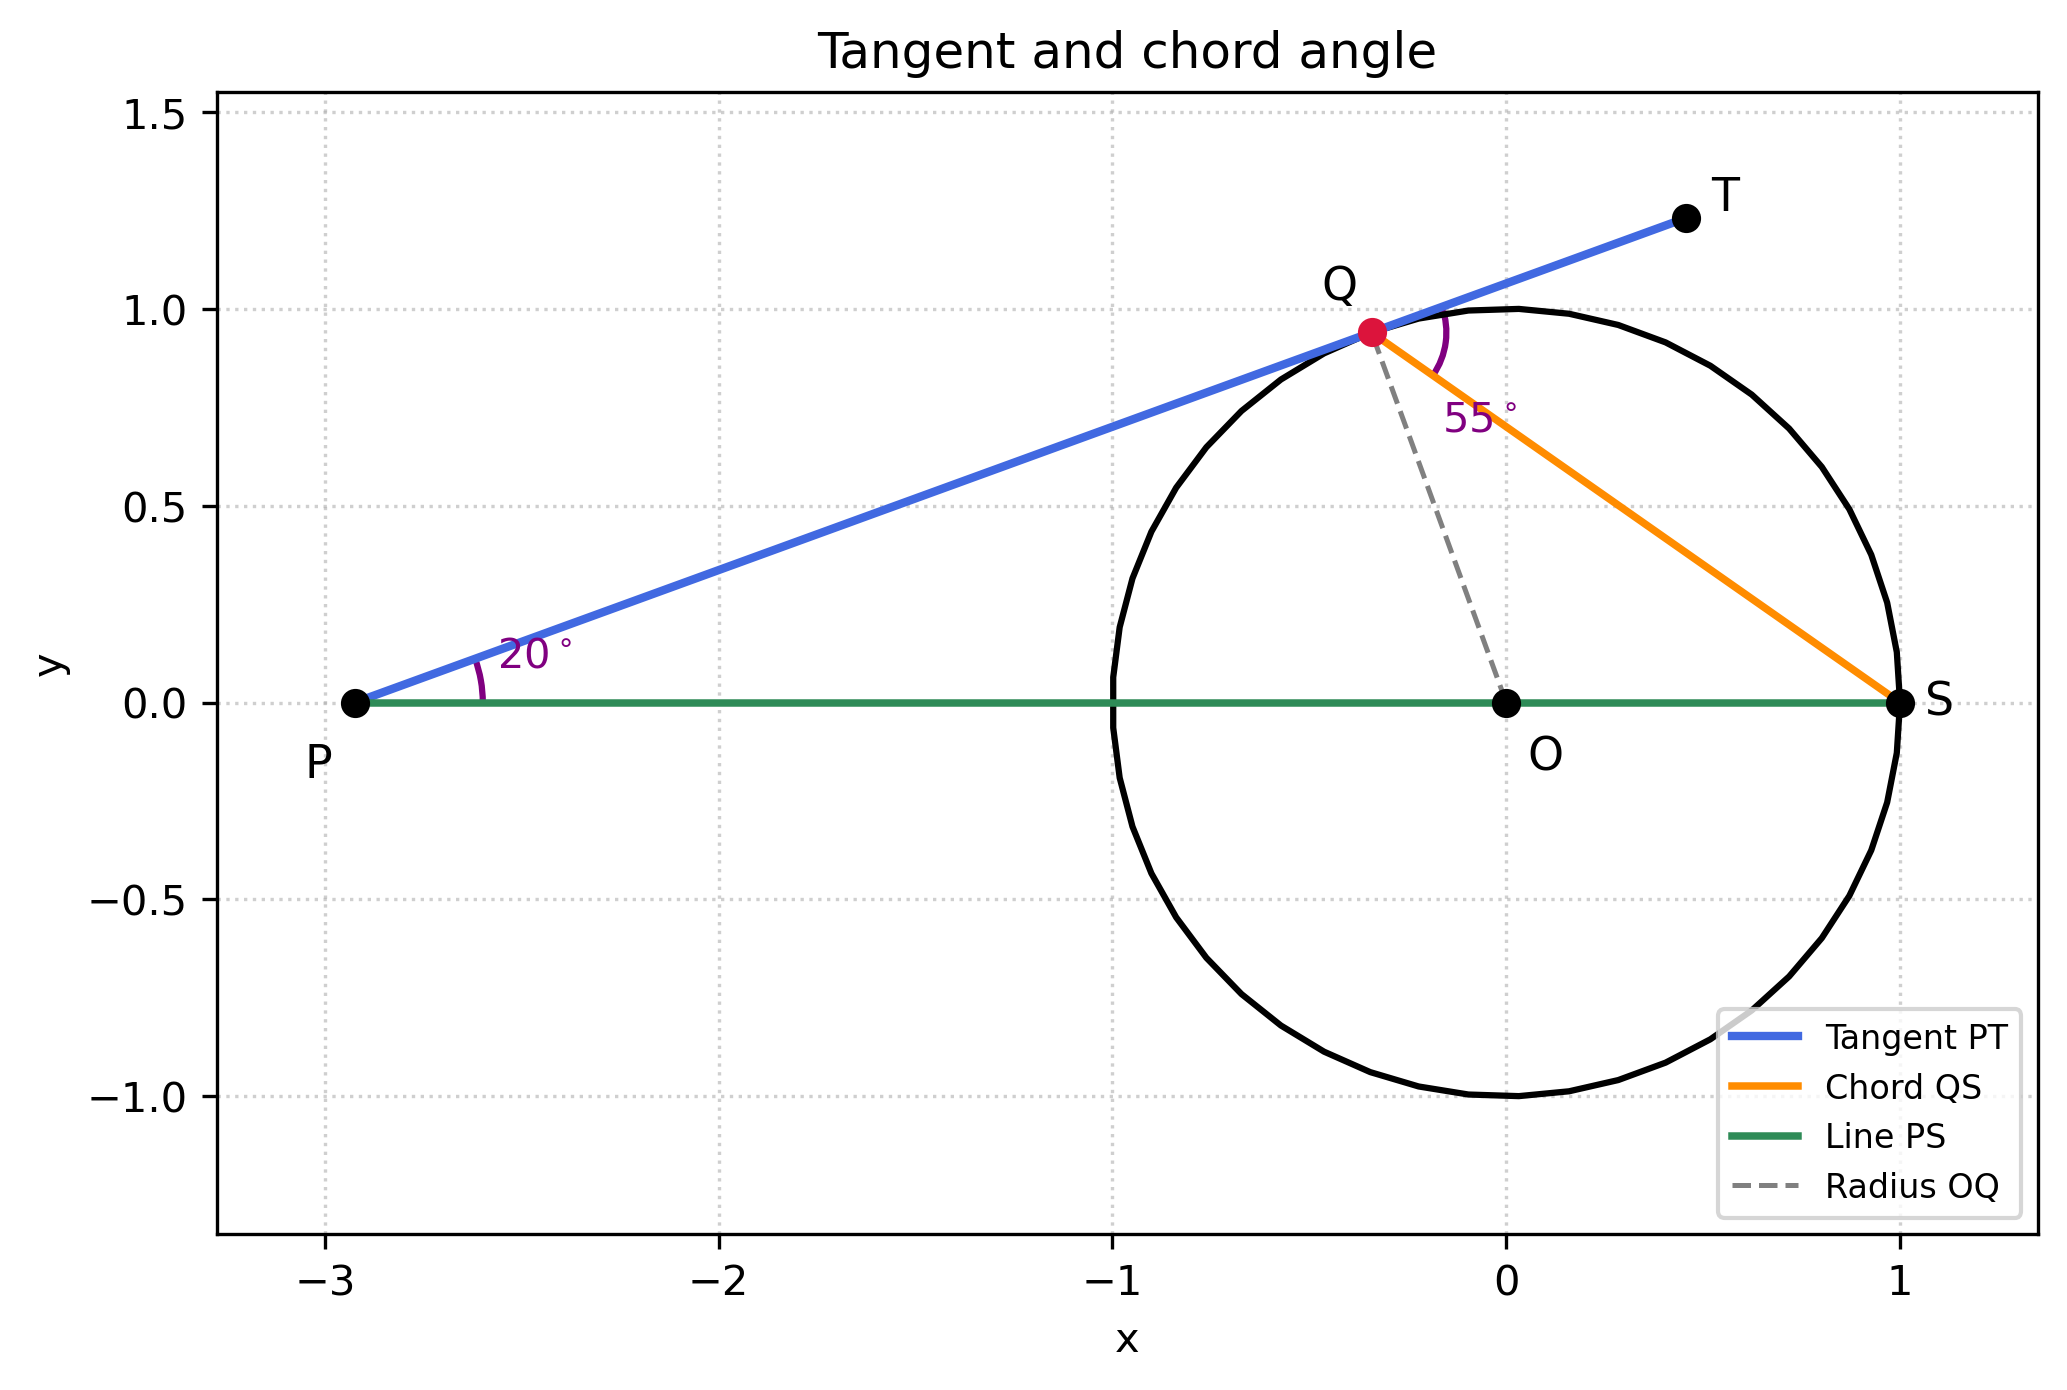
\includegraphics[width=0.60\linewidth]{figs/5.1.4.png}
    \caption{Tangent-chord configuration for Question 4.}
    \label{fig:q4-graph}
\end{figure}


\end{list}
\vspace{1.2em}
\begin{list}{}{\setlength{\leftmargin}{1.15cm}\setlength{\labelwidth}{1.0cm}\setlength{\labelsep}{0.15cm}\setlength{\itemindent}{0pt}\setlength{\listparindent}{0pt}\setlength{\parsep}{0pt}\setlength{\topsep}{0pt}}\setlist[enumerate]{leftmargin=0.7cm}
\item[5.1.5] Devansh proved that $\triangle ABC \sim \triangle PQR$ using the SAS similarity criterion. If $\angle C = \angle R$, which of the following statements was proved true?

\begin{enumerate}
    \item[(A)] $\dfrac{AC}{AB} = \dfrac{PR}{PQ}$
    \item[(B)] $\dfrac{BC}{AC} = \dfrac{PR}{QR}$
    \item[(C)] $\dfrac{AC}{BC} = \dfrac{PR}{PQ}$
    \item[(D)] $\dfrac{AC}{BC} = \dfrac{PR}{QR}$
\end{enumerate}

\vspace{0.7em}\par\noindent\textbf{Solution:}

The equal angles $\angle C$ and $\angle R$ are included between the pairs of sides $AC, BC$ and $PR, QR$, respectively. By the SAS similarity criterion, the corresponding sides are proportional:
\[
\frac{AC}{PR} = \frac{BC}{QR}.
\]
Rearranging,
\[
\frac{AC}{BC} = \frac{PR}{QR}.
\]
Therefore, the correct answer is \textbf{(D)}.


\end{list}
\vspace{1.2em}
\begin{list}{}{\setlength{\leftmargin}{1.15cm}\setlength{\labelwidth}{1.0cm}\setlength{\labelsep}{0.15cm}\setlength{\itemindent}{0pt}\setlength{\listparindent}{0pt}\setlength{\parsep}{0pt}\setlength{\topsep}{0pt}}\setlist[enumerate]{leftmargin=0.7cm}
\item[5.1.6] While calculating the mean of a grouped frequency distribution, the step-deviation method $\left(\frac{x_i-a}{h}=u_i\right)$ was used. It was found that $\bar{x}=64$, $h=5$, and $a=62.5$. The value of $\bar{u}$ is:

\begin{enumerate}
    \item[(A)] $0.5$
    \item[(B)] $1.5$
    \item[(C)] $0.3$
    \item[(D)] $7.5$
\end{enumerate}

\vspace{0.7em}\par\noindent\textbf{Solution:}

Using the step-deviation relation,
\[
\bar{u}=\frac{\bar{x}-a}{h}=\frac{64-62.5}{5}=0.3.
\]
The correct answer is \textbf{(C)}.

\end{list}
\vspace{1.2em}
\begin{list}{}{\setlength{\leftmargin}{1.15cm}\setlength{\labelwidth}{1.0cm}\setlength{\labelsep}{0.15cm}\setlength{\itemindent}{0pt}\setlength{\listparindent}{0pt}\setlength{\parsep}{0pt}\setlength{\topsep}{0pt}}\setlist[enumerate]{leftmargin=0.7cm}
\item[5.1.7] A conical cavity of maximum volume is carved out from a wooden solid hemisphere of radius $10$ cm. The curved surface area of the cavity carved out is (use $\pi=3.14$):

\begin{enumerate}
    \item[(A)] $314\sqrt{2}\text{ cm}^2$
    \item[(B)] $314\text{ cm}^2$
    \item[(C)] $\dfrac{3140}{3}\text{ cm}^2$
    \item[(D)] $3140\sqrt{2}\text{ cm}^2$
\end{enumerate}

\vspace{0.7em}\par\noindent\textbf{Solution:}

For the maximum-volume cone shown by the hemisphere's dimensions, the base radius and height are both $10$ cm. Its slant height is
\[
\ell=\sqrt{10^2+10^2}=10\sqrt{2}\text{ cm}.
\]
Therefore, the curved surface area is
\[
\pi r\ell=3.14\times 10\times 10\sqrt{2}=314\sqrt{2}\text{ cm}^2.
\]
The correct answer is \textbf{(A)}.

\end{list}
\vspace{1.2em}
\begin{list}{}{\setlength{\leftmargin}{1.15cm}\setlength{\labelwidth}{1.0cm}\setlength{\labelsep}{0.15cm}\setlength{\itemindent}{0pt}\setlength{\listparindent}{0pt}\setlength{\parsep}{0pt}\setlength{\topsep}{0pt}}\setlist[enumerate]{leftmargin=0.7cm}
\item[5.1.8] If $a_n$ represents the $n$th term of the A.P. $-\dfrac{15}{4},-\dfrac{10}{4},-\dfrac{5}{4},\ldots$, then the value of $a_{16}-a_{12}$ is:

\begin{enumerate}
    \item[(A)] $4$
    \item[(B)] $\dfrac{5}{4}$
    \item[(C)] $5$
    \item[(D)] $\dfrac{25}{4}$
\end{enumerate}

\vspace{0.7em}\par\noindent\textbf{Solution:}

The first term is $a_1=-\dfrac{15}{4}$ and the common difference is $d=\dfrac{5}{4}$. Hence,
\[
a_n=a_1+(n-1)d=\frac{5n-20}{4}.
\]
Therefore,
\[
a_{16}-a_{12}=\frac{5(16)-20}{4}-\frac{5(12)-20}{4}=15-10=5.
\]
The correct answer is \textbf{(C)}.

The following C program computes the $n$th term and evaluates the requested difference:
\begin{lstlisting}[frame=single, basicstyle=\rmfamily, escapeinside={(*@}{@*)}]
(*@\makebox[\dimexpr\linewidth-2\fboxsep-2\fboxrule\relax][c]{codes/5.1.8.c}@*)
\end{lstlisting}

\end{list}
\vspace{1.2em}
\begin{list}{}{\setlength{\leftmargin}{1.15cm}\setlength{\labelwidth}{1.0cm}\setlength{\labelsep}{0.15cm}\setlength{\itemindent}{0pt}\setlength{\listparindent}{0pt}\setlength{\parsep}{0pt}\setlength{\topsep}{0pt}}\setlist[enumerate]{leftmargin=0.7cm}
\item[5.1.9] The value of $p$ for which the roots of the quadratic equation $x^2-px+6=0$ are rational is:

\begin{enumerate}
    \item[(A)] $1$
    \item[(B)] $-5$
    \item[(C)] $25$
    \item[(D)] $\sqrt{5}$
\end{enumerate}

\vspace{0.7em}\par\noindent\textbf{Solution:}

For $p=-5$, the equation becomes
\[
x^2+5x+6=(x+2)(x+3)=0,
\]
so its roots are $-2$ and $-3$, both rational. The other listed values do not give two rational roots. Therefore, the correct answer is \textbf{(B)}.

The following code generates the graph shown below.
\begin{lstlisting}[frame=single, basicstyle=\rmfamily, escapeinside={(*@}{@*)}]
(*@\makebox[\dimexpr\linewidth-2\fboxsep-2\fboxrule\relax][c]{codes/5.1.9.py}@*)
\end{lstlisting}
\begin{figure}[H]
    \centering
    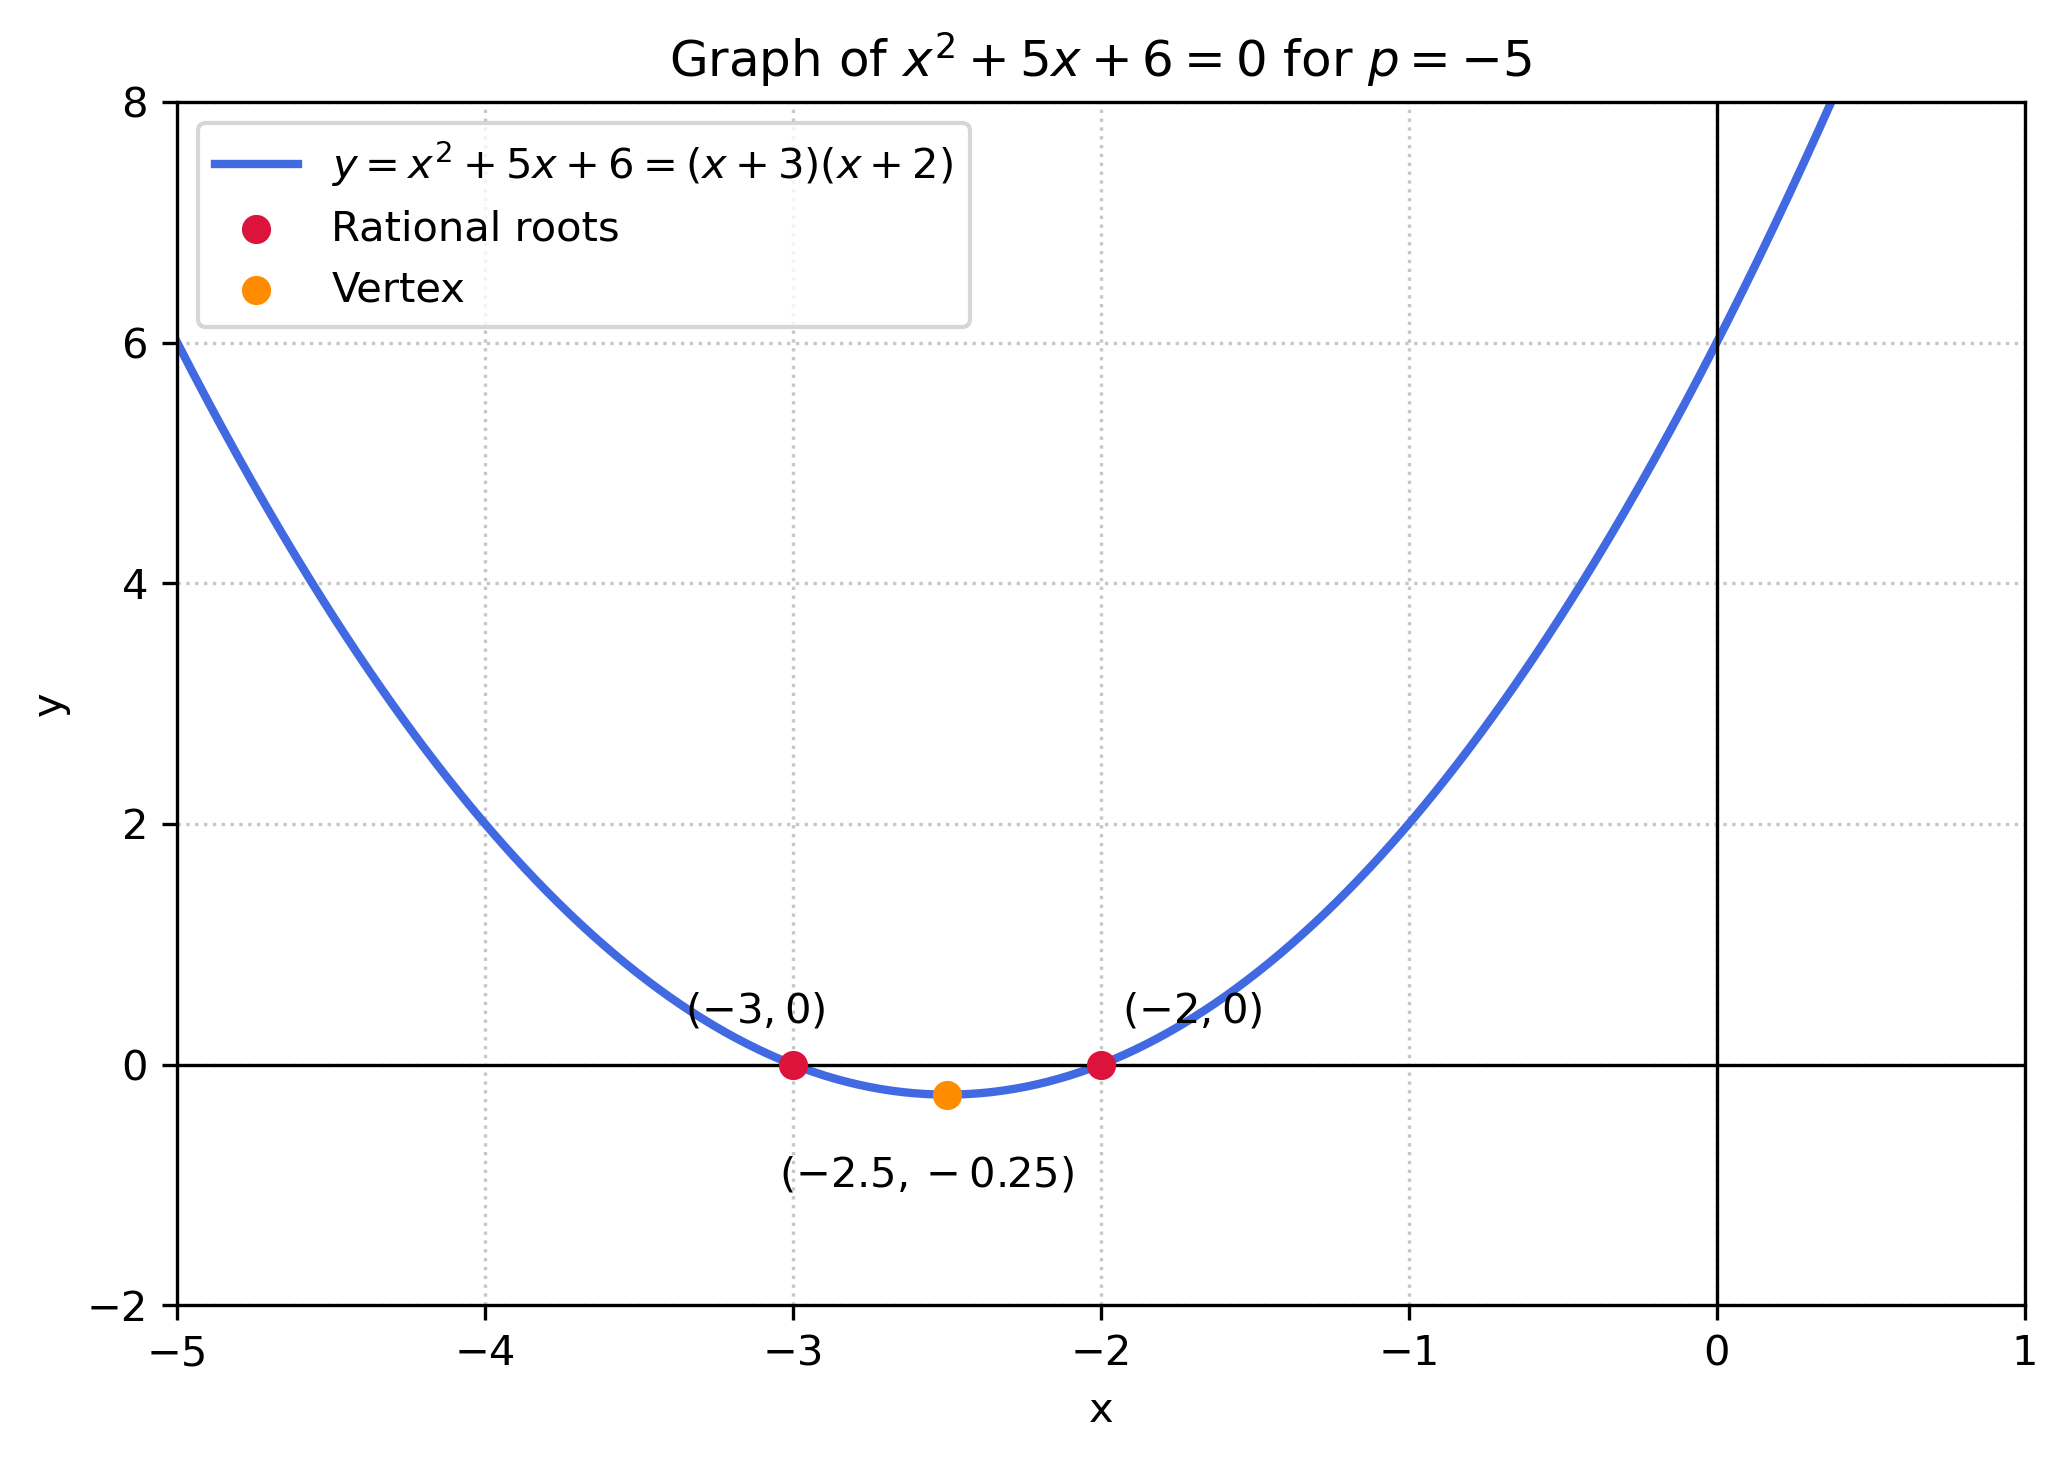
\includegraphics[width=0.48\linewidth]{figs/5.1.9.png}
    \caption{Graph of $y=x^2+5x+6$, whose roots are $-3$ and $-2$.}
    \label{fig:q9-graph}
\end{figure}
\begin{list}{}{\setlength{\leftmargin}{1.15cm}\setlength{\labelwidth}{1.0cm}\setlength{\labelsep}{0.15cm}\setlength{\itemindent}{0pt}\setlength{\listparindent}{0pt}\setlength{\parsep}{0pt}\setlength{\topsep}{0pt}}\setlist[enumerate]{leftmargin=0.7cm}
\item[5.1.11] A card is drawn at random from a well-shuffled deck of 52 playing cards. Find the probability that it is either a ten or a king.

\vspace{0.7em}\par\noindent\textbf{Solution:} There are 8 favorable cards, so the probability is $\dfrac{8}{52}=\dfrac{2}{13}$. The answer is \textbf{(B)}.
\end{list}
\vspace{1.2em}
\begin{list}{}{\setlength{\leftmargin}{1.15cm}\setlength{\labelwidth}{1.0cm}\setlength{\labelsep}{0.15cm}\setlength{\itemindent}{0pt}\setlength{\listparindent}{0pt}\setlength{\parsep}{0pt}\setlength{\topsep}{0pt}}\setlist[enumerate]{leftmargin=0.7cm}
\item[5.1.14] For an acute angle $\theta$, if $\sin\theta=\dfrac{1}{9}$, find the value of $\dfrac{9\operatorname{cosec}\theta+1}{9\operatorname{cosec}\theta-1}$.

\vspace{0.7em}\par\noindent\textbf{Solution:} Since $\operatorname{cosec}\theta=9$, the value is $\dfrac{82}{80}=\dfrac{41}{40}$. The correct answer is \textbf{(D)}.
\end{list}
\vspace{1.2em}
\begin{list}{}{\setlength{\leftmargin}{1.15cm}\setlength{\labelwidth}{1.0cm}\setlength{\labelsep}{0.15cm}\setlength{\itemindent}{0pt}\setlength{\listparindent}{0pt}\setlength{\parsep}{0pt}\setlength{\topsep}{0pt}}\setlist[enumerate]{leftmargin=0.7cm}
\item[5.1.15] In the given figure, $PQ\parallel YZ$ and $XP:PY=2:3$. If $PQ=5$ cm, find $YZ$.

\vspace{0.7em}\par\noindent\textbf{Solution:} $XY:XP=5:2$. By similarity, $YZ:PQ=XY:XP=5:2$, so $YZ=12.5$ cm. The correct answer is \textbf{(A)}.
\end{list}
\vspace{1.2em}
\begin{list}{}{\setlength{\leftmargin}{1.15cm}\setlength{\labelwidth}{1.0cm}\setlength{\labelsep}{0.15cm}\setlength{\itemindent}{0pt}\setlength{\listparindent}{0pt}\setlength{\parsep}{0pt}\setlength{\topsep}{0pt}}\setlist[enumerate]{leftmargin=0.7cm}
\item[5.1.16] Meena's probability of winning the first prize in a lottery is $0.08$. If 800 tickets were sold, how many tickets did she buy?

\vspace{0.7em}\par\noindent\textbf{Solution:} Number of tickets $=0.08\times800=64$. The correct answer is \textbf{(A)}.
\end{list}
\vspace{1.2em}
\begin{list}{}{\setlength{\leftmargin}{1.15cm}\setlength{\labelwidth}{1.0cm}\setlength{\labelsep}{0.15cm}\setlength{\itemindent}{0pt}\setlength{\listparindent}{0pt}\setlength{\parsep}{0pt}\setlength{\topsep}{0pt}}\setlist[enumerate]{leftmargin=0.7cm}
\item[5.1.19] Assertion (A): The system $3x-5y+7=0$ and $-6x+10y+14=0$ is inconsistent.\\
Reason (R): When two linear equations do not have a unique solution, they always represent parallel lines.

\vspace{0.7em}\par\noindent\textbf{Solution:} The equations reduce to $y=\frac35x+\frac75$ and $y=\frac35x-\frac75$. They are distinct parallel lines, so the assertion is true. The reason is false because coincident lines also have no unique solution. The correct choice is \textbf{(C)} (A is true, R is false).

\begin{lstlisting}[frame=single, basicstyle=\rmfamily, escapeinside={(*@}{@*)}]
(*@\makebox[\dimexpr\linewidth-2\fboxsep-2\fboxrule\relax][c]{codes/5.1.19.py}@*)
\end{lstlisting}
The graph shows the two parallel lines.
\begin{figure}[H]
\centering
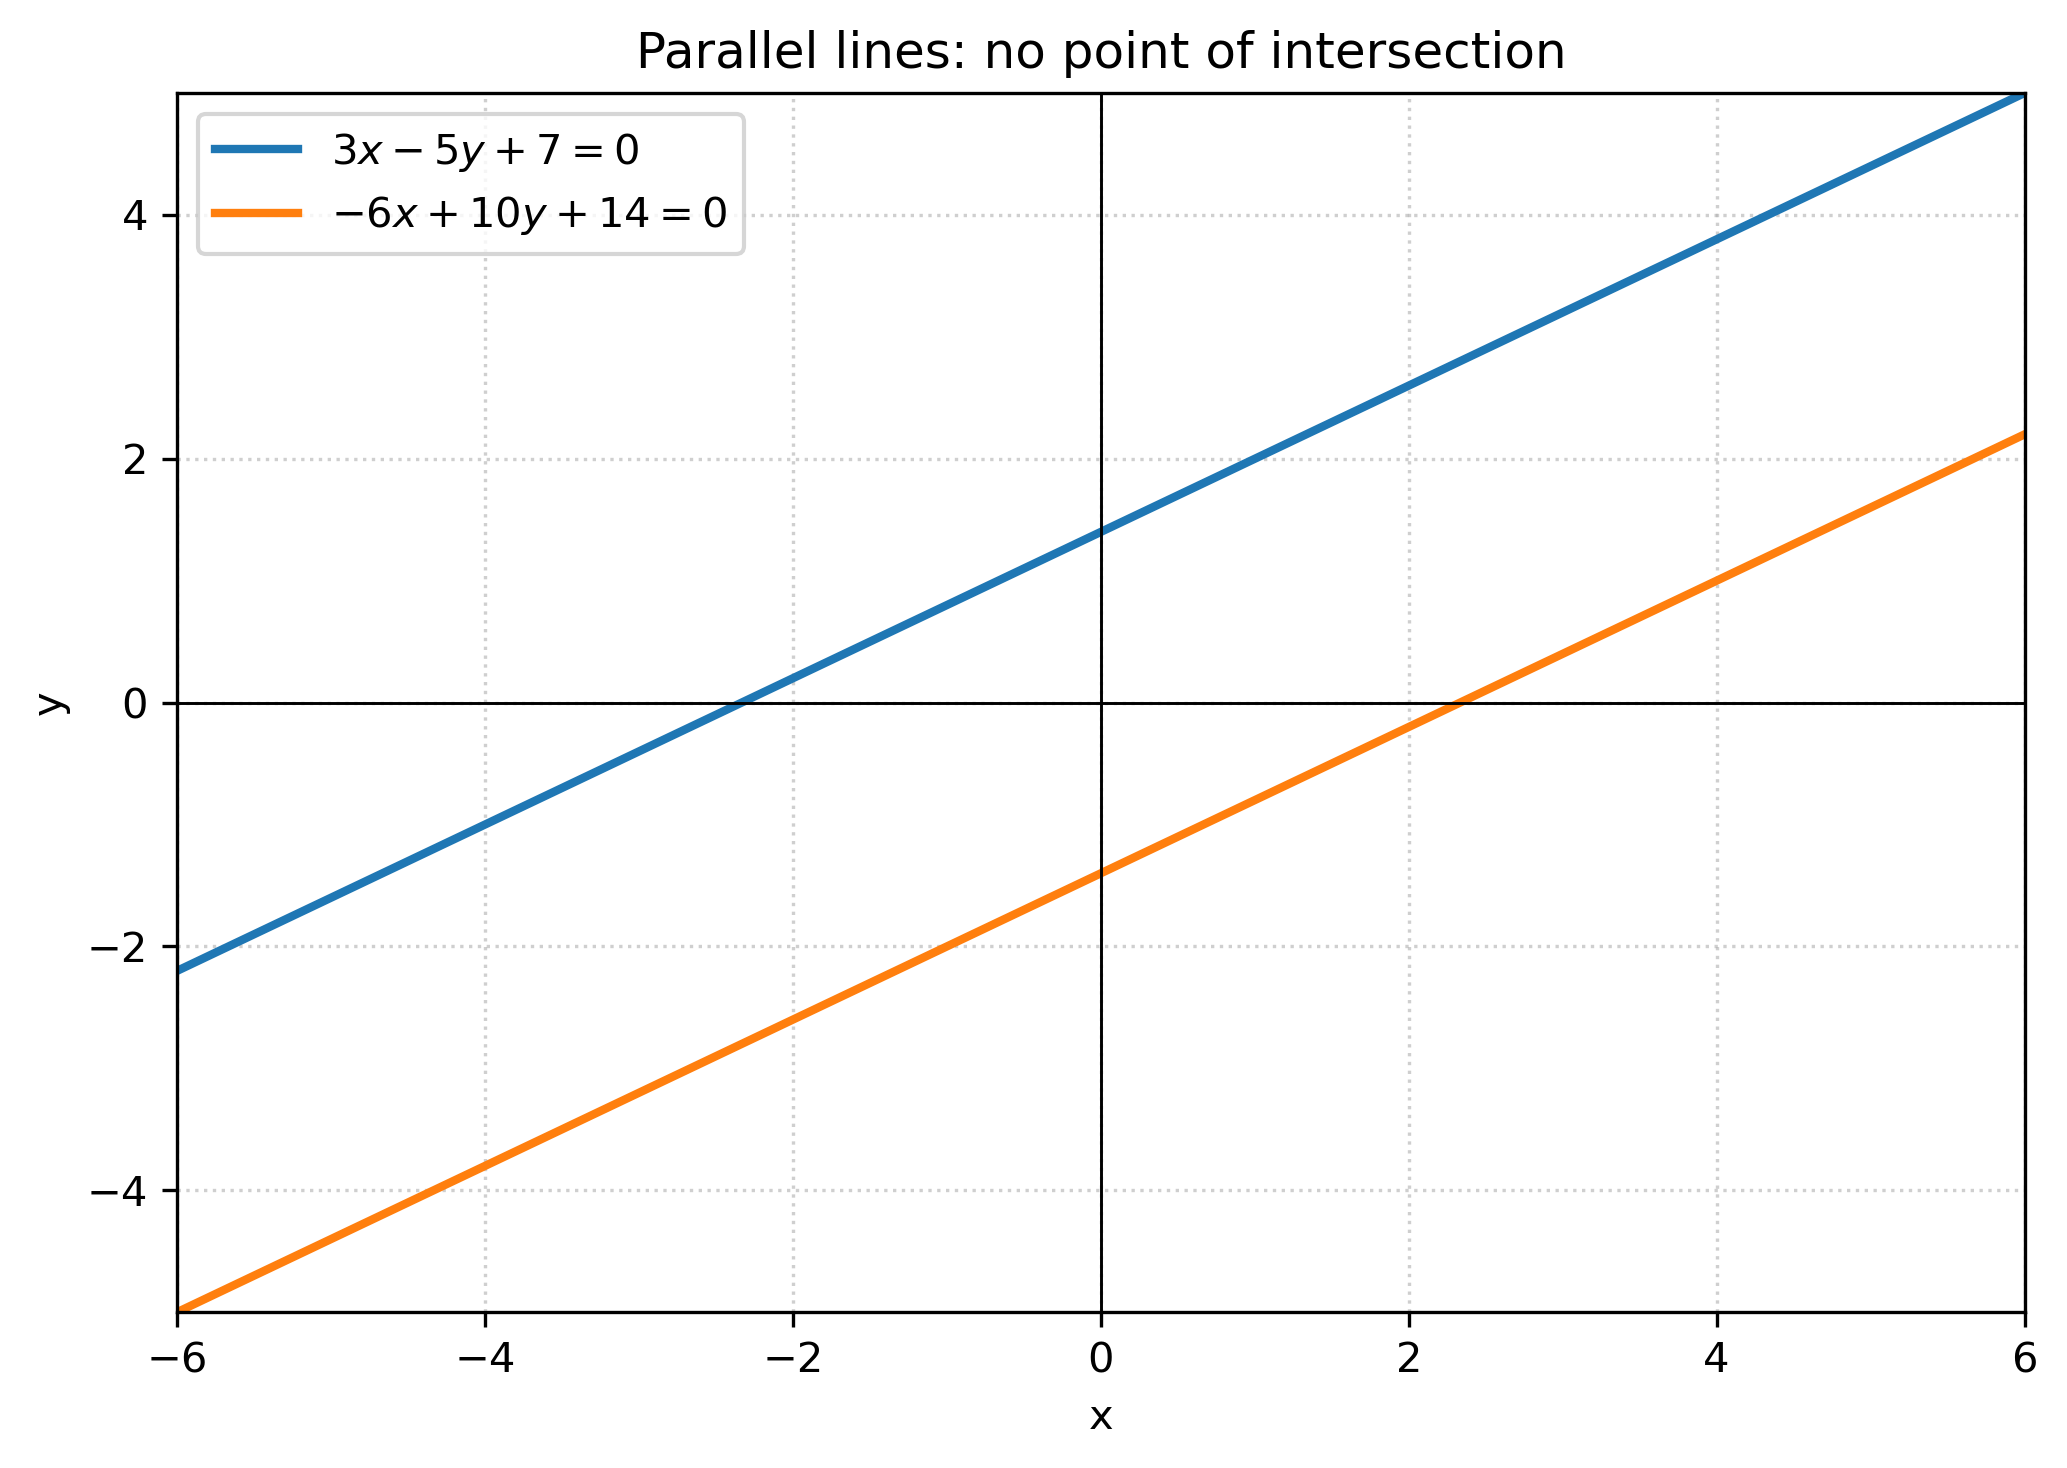
\includegraphics[width=0.56\linewidth]{figs/5.1.19.png}
\caption{The two distinct parallel lines in Question 19.}
\label{fig:q19}
\end{figure}
\end{list}
\vspace{1.2em}
\begin{list}{}{\setlength{\leftmargin}{1.15cm}\setlength{\labelwidth}{1.0cm}\setlength{\labelsep}{0.15cm}\setlength{\itemindent}{0pt}\setlength{\listparindent}{0pt}\setlength{\parsep}{0pt}\setlength{\topsep}{0pt}}\setlist[enumerate]{leftmargin=0.7cm}
\item[5.1.22.1] The vertices of right triangle $ABC$, with $\angle B=90^\circ$, are $A(3,4)$, $B(1,1)$ and $C(-8,7)$. Find $\tan A$.

\vspace{0.7em}\par\noindent\textbf{Solution:} $AB=\sqrt{13}$ and $BC=3\sqrt{13}$. Hence $\tan A=\dfrac{BC}{AB}=3$.

\begin{lstlisting}[frame=single, basicstyle=\rmfamily, escapeinside={(*@}{@*)}]
(*@\makebox[\dimexpr\linewidth-2\fboxsep-2\fboxrule\relax][c]{codes/5.1.22.1.py}@*)
\end{lstlisting}
\begin{figure}[H]
\centering
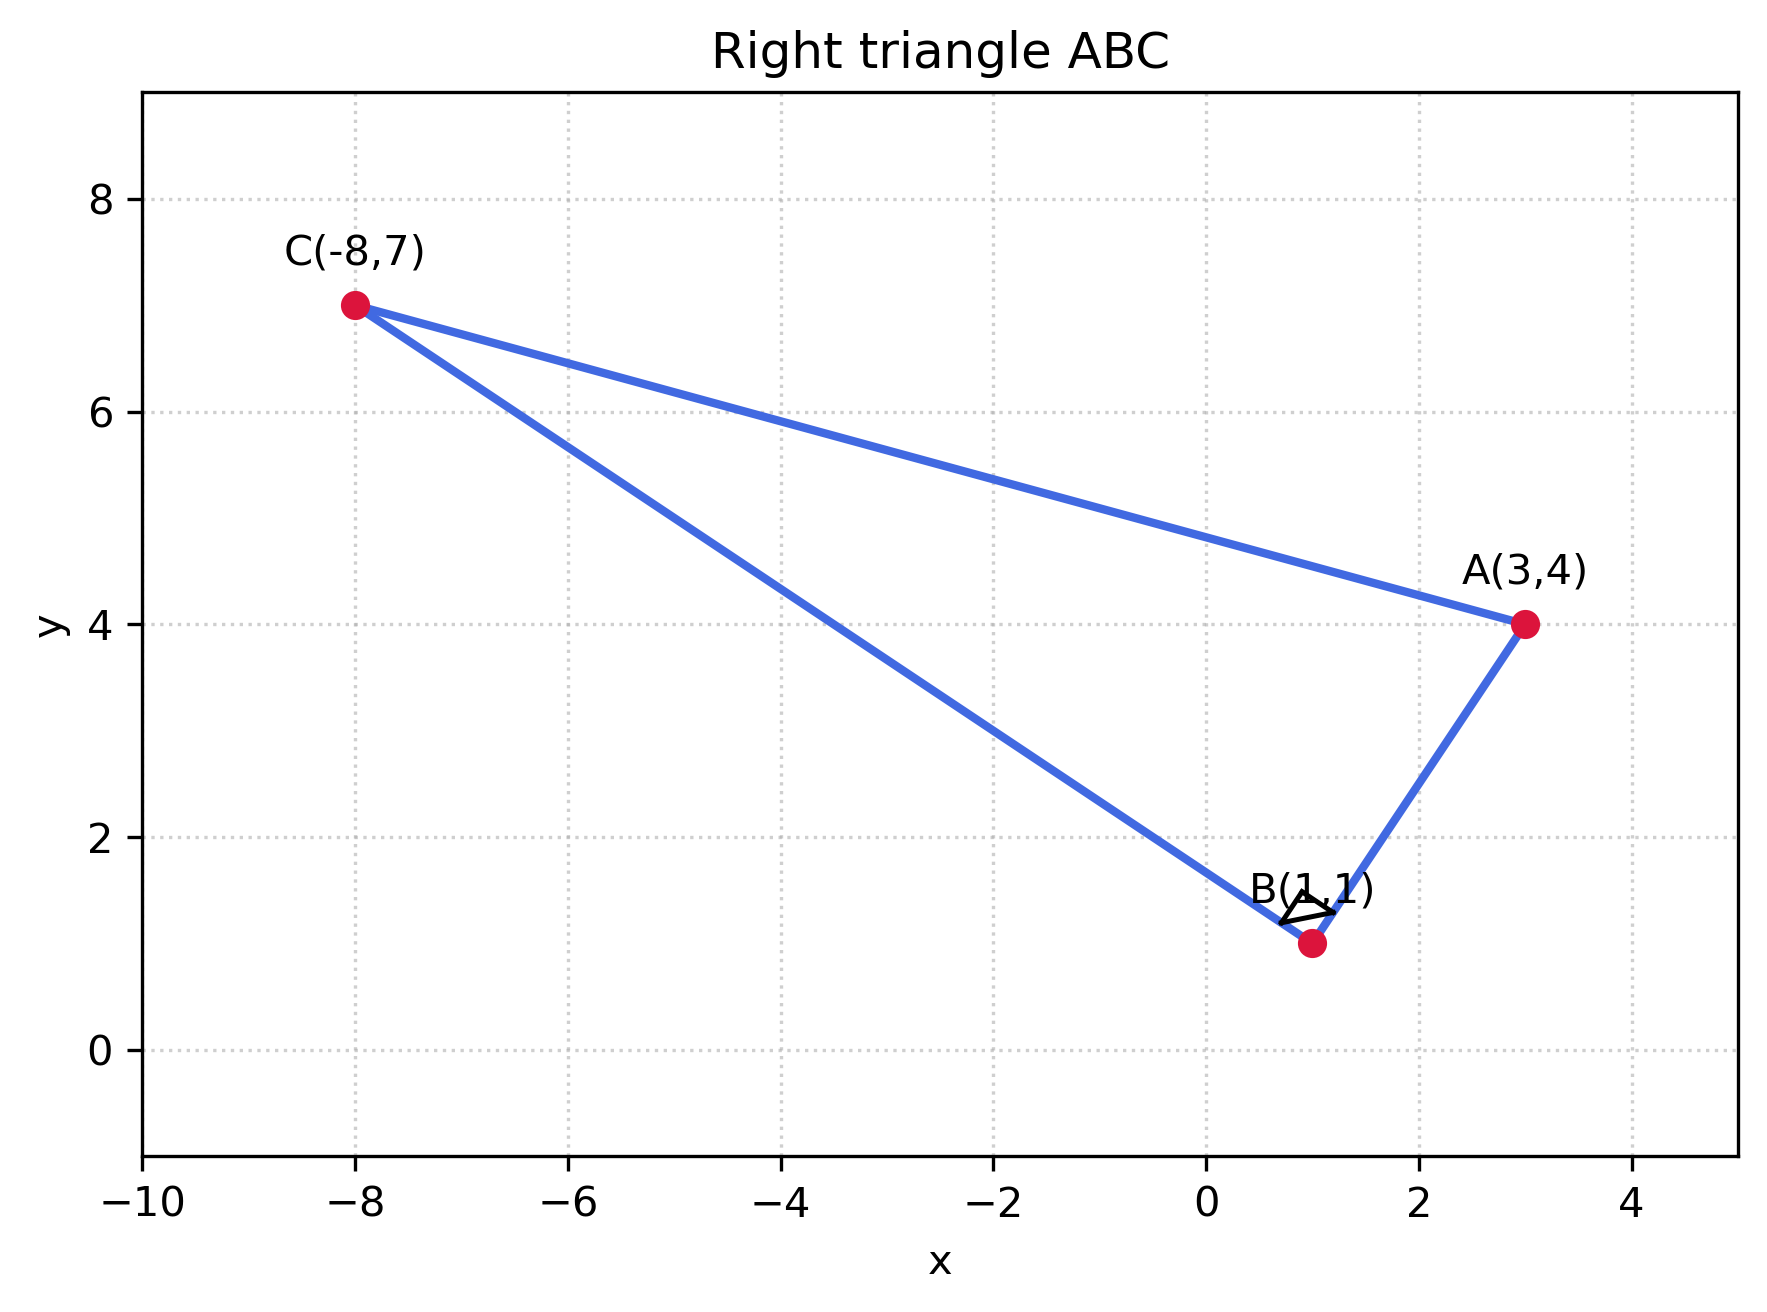
\includegraphics[width=0.52\linewidth]{figs/5.1.22.1.png}
\caption{Triangle $ABC$ plotted from the given vertices.}
\label{fig:q22a}
\end{figure}
\end{list}
\vspace{1.2em}
\begin{list}{}{\setlength{\leftmargin}{1.15cm}\setlength{\labelwidth}{1.0cm}\setlength{\labelsep}{0.15cm}\setlength{\itemindent}{0pt}\setlength{\listparindent}{0pt}\setlength{\parsep}{0pt}\setlength{\topsep}{0pt}}\setlist[enumerate]{leftmargin=0.7cm}
\item[5.1.23] In the given figure, $AB\parallel DE$ and $AC\parallel DF$. If $BC=10$ cm, $EB=CF=5$ cm and $AB=7$ cm, find $DE$.

\vspace{0.7em}\par\noindent\textbf{Solution:} $EF=EB+BC+CF=20$ cm. Since $\triangle ABC\sim\triangle DEF$, $\dfrac{DE}{AB}=\dfrac{EF}{BC}=2$, so $DE=14$ cm.

\begin{lstlisting}[frame=single, basicstyle=\rmfamily, escapeinside={(*@}{@*)}]
(*@\makebox[\dimexpr\linewidth-2\fboxsep-2\fboxrule\relax][c]{codes/5.1.23.py}@*)
\end{lstlisting}
This code recreates the diagram in the question.
\begin{figure}[H]
\centering
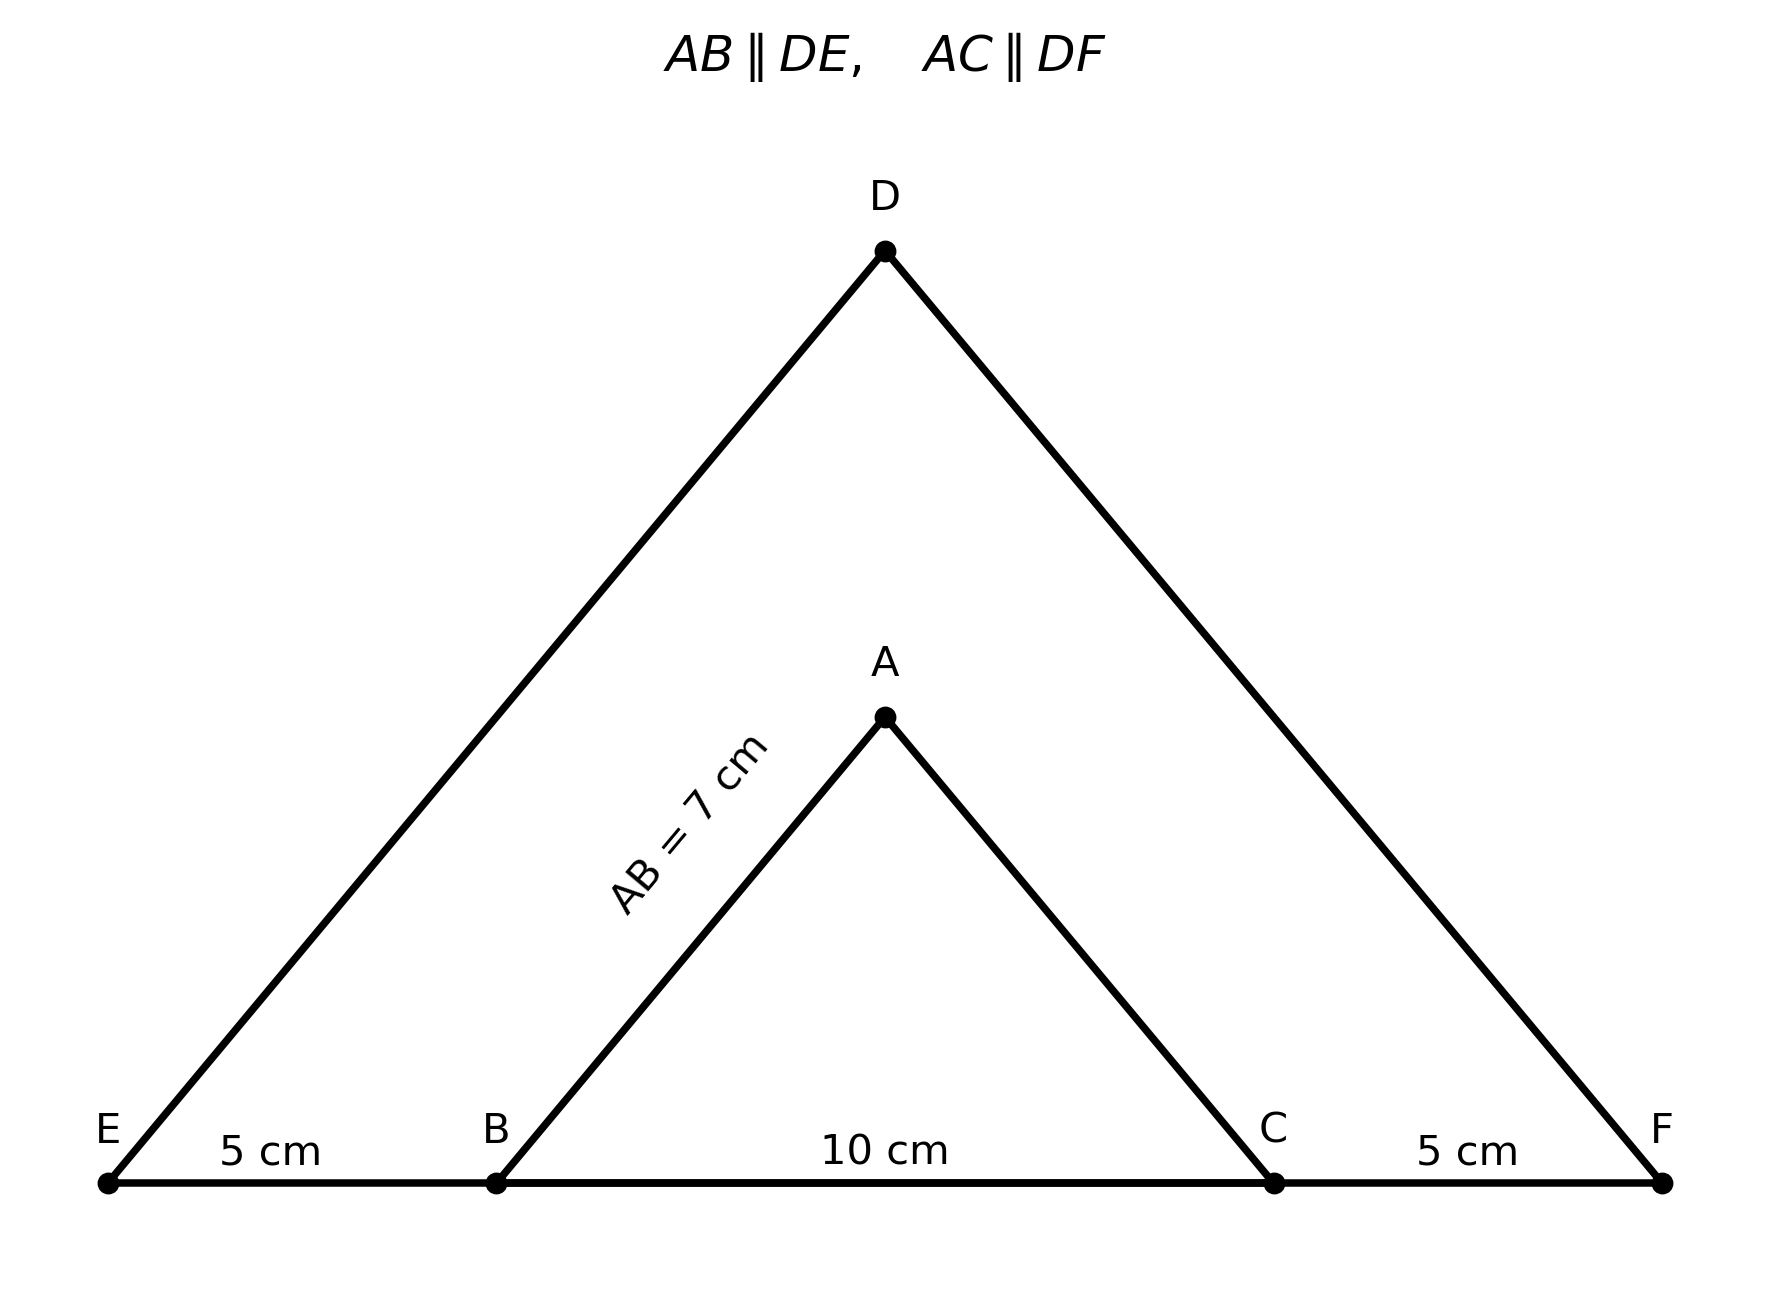
\includegraphics[width=0.46\linewidth]{figs/5.1.23.png}
\caption{Recreated configuration for Question 23.}
\label{fig:q23}
\end{figure}
\end{list}
\vspace{1.2em}
\begin{list}{}{\setlength{\leftmargin}{1.15cm}\setlength{\labelwidth}{1.0cm}\setlength{\labelsep}{0.15cm}\setlength{\itemindent}{0pt}\setlength{\listparindent}{0pt}\setlength{\parsep}{0pt}\setlength{\topsep}{0pt}}\setlist[enumerate]{leftmargin=0.7cm}
\item[5.1.26] A circle of diameter 20 cm is divided equally into five sectors. Find the area and perimeter of one sector.

\vspace{0.7em}\par\noindent\textbf{Solution:} The radius is 10 cm and the central angle is $72^\circ$. The area is $\dfrac{72}{360}\pi(10)^2=20\pi$ cm$^2$. The perimeter is $2(10)+\dfrac{72}{360}(2\pi\cdot10)=20+4\pi$ cm.

\begin{lstlisting}[frame=single, basicstyle=\rmfamily, escapeinside={(*@}{@*)}]
(*@\makebox[\dimexpr\linewidth-2\fboxsep-2\fboxrule\relax][c]{codes/5.1.26.py}@*)
\end{lstlisting}
\begin{figure}[H]
\centering
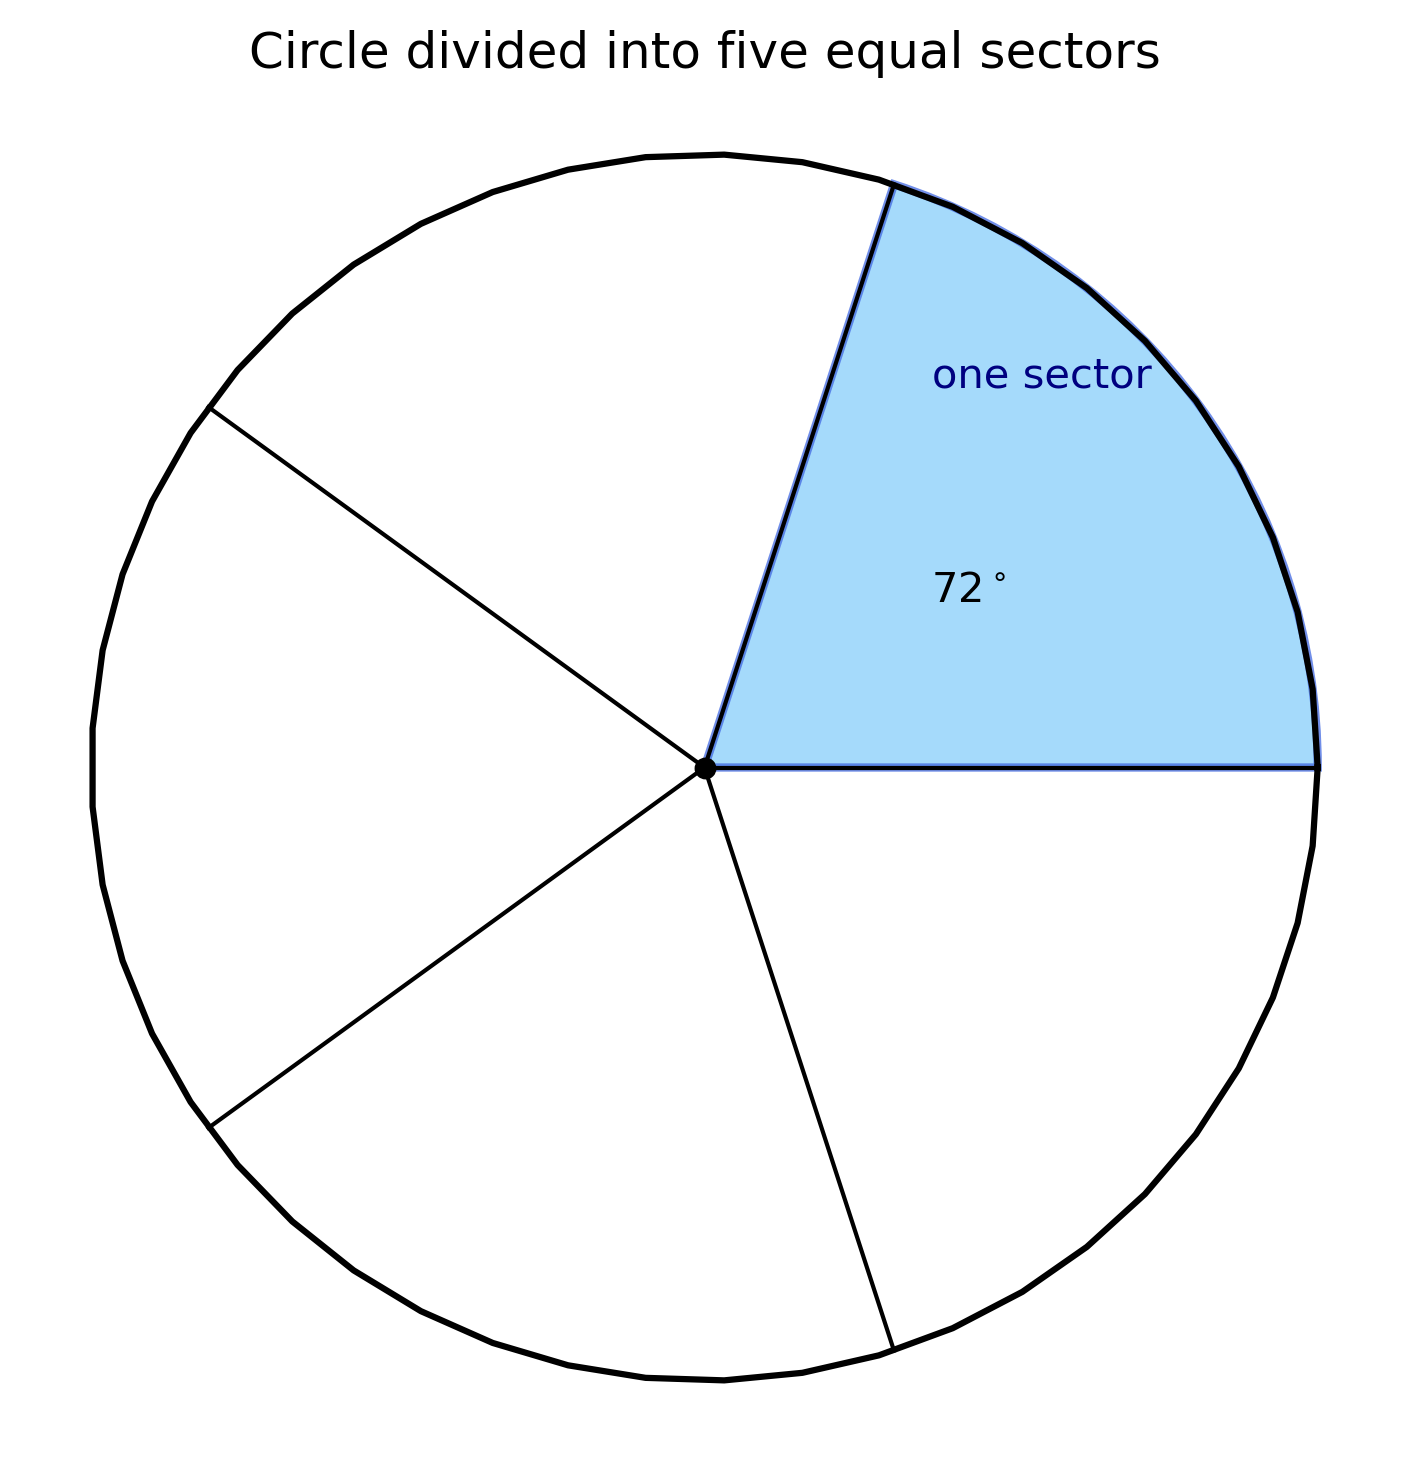
\includegraphics[width=0.32\linewidth]{figs/5.1.26.png}
\caption{One of the five equal sectors highlighted.}
\label{fig:q26}
\end{figure}
\end{list}
\vspace{1.2em}
\begin{list}{}{\setlength{\leftmargin}{1.15cm}\setlength{\labelwidth}{1.0cm}\setlength{\labelsep}{0.15cm}\setlength{\itemindent}{0pt}\setlength{\listparindent}{0pt}\setlength{\parsep}{0pt}\setlength{\topsep}{0pt}}\setlist[enumerate]{leftmargin=0.7cm}
\item[5.1.27.2] The sum of the first $n$ terms of an A.P. is $S_n=2n^2+13n$. Find its $n$th term and hence its 10th term.

\vspace{0.7em}\par\noindent\textbf{Solution:} $a_n=S_n-S_{n-1}=4n+11$, so $a_{10}=51$.

The C program calculates the $n$th term for any positive integer $n$.

\begin{lstlisting}[frame=single, basicstyle=\rmfamily, escapeinside={(*@}{@*)}]
(*@\makebox[\dimexpr\linewidth-2\fboxsep-2\fboxrule\relax][c]{codes/5.1.27.2.c}@*)
\end{lstlisting}
\end{list}
\vspace{1.2em}
\begin{list}{}{\setlength{\leftmargin}{1.15cm}\setlength{\labelwidth}{1.0cm}\setlength{\labelsep}{0.15cm}\setlength{\itemindent}{0pt}\setlength{\listparindent}{0pt}\setlength{\parsep}{0pt}\setlength{\topsep}{0pt}}\setlist[enumerate]{leftmargin=0.7cm}
\item[5.1.29.1] A circle centred at $(2,1)$ passes through $A(5,6)$ and $B(-3,K)$. Find the possible values of $K$ and the length of chord $AB$ in each case.

\vspace{0.7em}\par\noindent\textbf{Solution:} The radius squared is $OA^2=34$. Thus $25+(K-1)^2=34$, giving $K=4$ or $K=-2$. The corresponding chord lengths are $2\sqrt{17}$ and $8\sqrt{2}$, respectively.

\begin{lstlisting}[frame=single, basicstyle=\rmfamily, escapeinside={(*@}{@*)}]
(*@\makebox[\dimexpr\linewidth-2\fboxsep-2\fboxrule\relax][c]{codes/5.1.29.1.py}@*)
\end{lstlisting}
\begin{figure}[H]
\centering
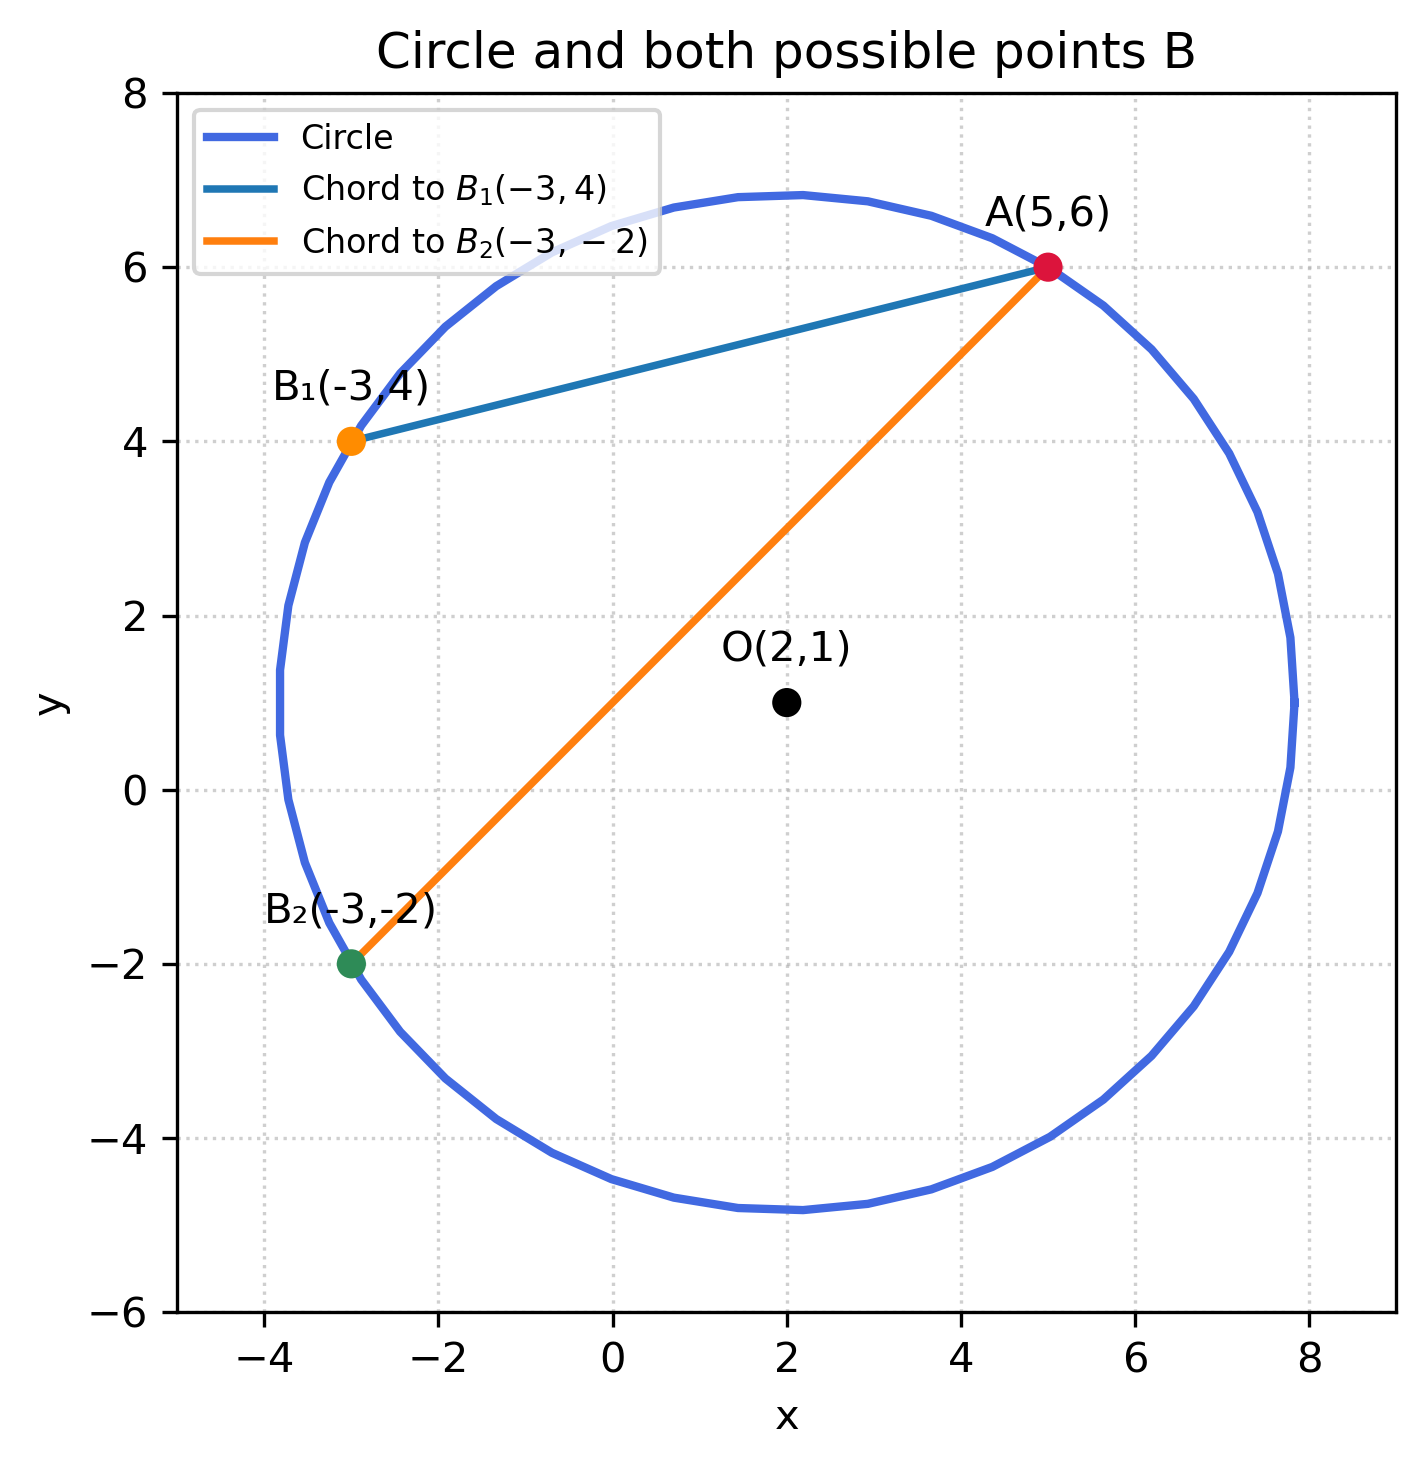
\includegraphics[width=0.38\linewidth]{figs/5.1.29.1.png}
\caption{The circle and both possible positions of $B$.}
\label{fig:q29a}
\end{figure}
\end{list}
\vspace{1.2em}
\begin{list}{}{\setlength{\leftmargin}{1.15cm}\setlength{\labelwidth}{1.0cm}\setlength{\labelsep}{0.15cm}\setlength{\itemindent}{0pt}\setlength{\listparindent}{0pt}\setlength{\parsep}{0pt}\setlength{\topsep}{0pt}}\setlist[enumerate]{leftmargin=0.7cm}
\item[5.1.29.2] Show that the point $P$ dividing the segment from $A(-1,7)$ to $B(4,-3)$ in the ratio $3:2$ lies on $x-3y=-1$. Find $PA$ and $PB$.

\vspace{0.7em}\par\noindent\textbf{Solution:} By the section formula, $P=(2,1)$, and $2-3(1)=-1$. Also, $PA=3\sqrt5$ and $PB=2\sqrt5$.

\begin{lstlisting}[frame=single, basicstyle=\rmfamily, escapeinside={(*@}{@*)}]
(*@\makebox[\dimexpr\linewidth-2\fboxsep-2\fboxrule\relax][c]{codes/5.1.29.2.py}@*)
\end{lstlisting}
\begin{figure}[H]
\centering
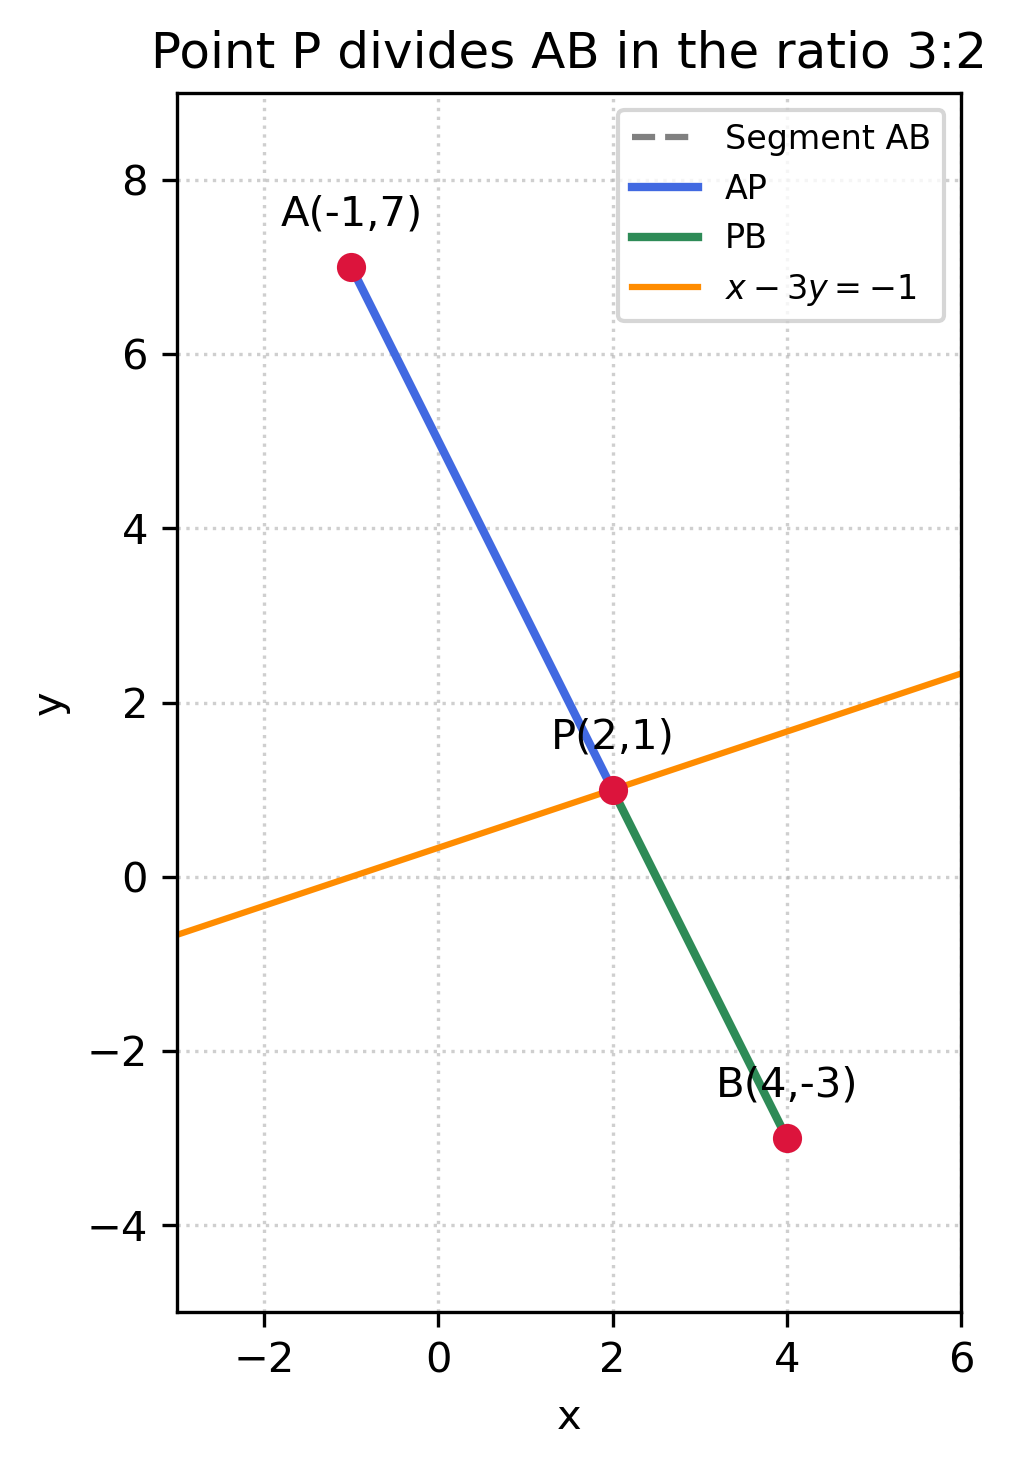
\includegraphics[width=0.27\linewidth]{figs/5.1.29.2.png}
\caption{Point $P$ on the line and segment $AB$.}
\label{fig:q29b}
\end{figure}
\end{list}
\vspace{1.2em}
\begin{list}{}{\setlength{\leftmargin}{1.15cm}\setlength{\labelwidth}{1.0cm}\setlength{\labelsep}{0.15cm}\setlength{\itemindent}{0pt}\setlength{\listparindent}{0pt}\setlength{\parsep}{0pt}\setlength{\topsep}{0pt}}\setlist[enumerate]{leftmargin=0.7cm}
\item[5.1.30] Solve graphically the system $x=4$ and $3x-2y=6$.

\vspace{0.7em}\par\noindent\textbf{Solution:} The lines intersect at $(4,3)$, so the solution is $x=4$, $y=3$.

\begin{lstlisting}[frame=single, basicstyle=\rmfamily, escapeinside={(*@}{@*)}]
(*@\makebox[\dimexpr\linewidth-2\fboxsep-2\fboxrule\relax][c]{codes/5.1.30.py}@*)
\end{lstlisting}
\begin{figure}[H]
\centering
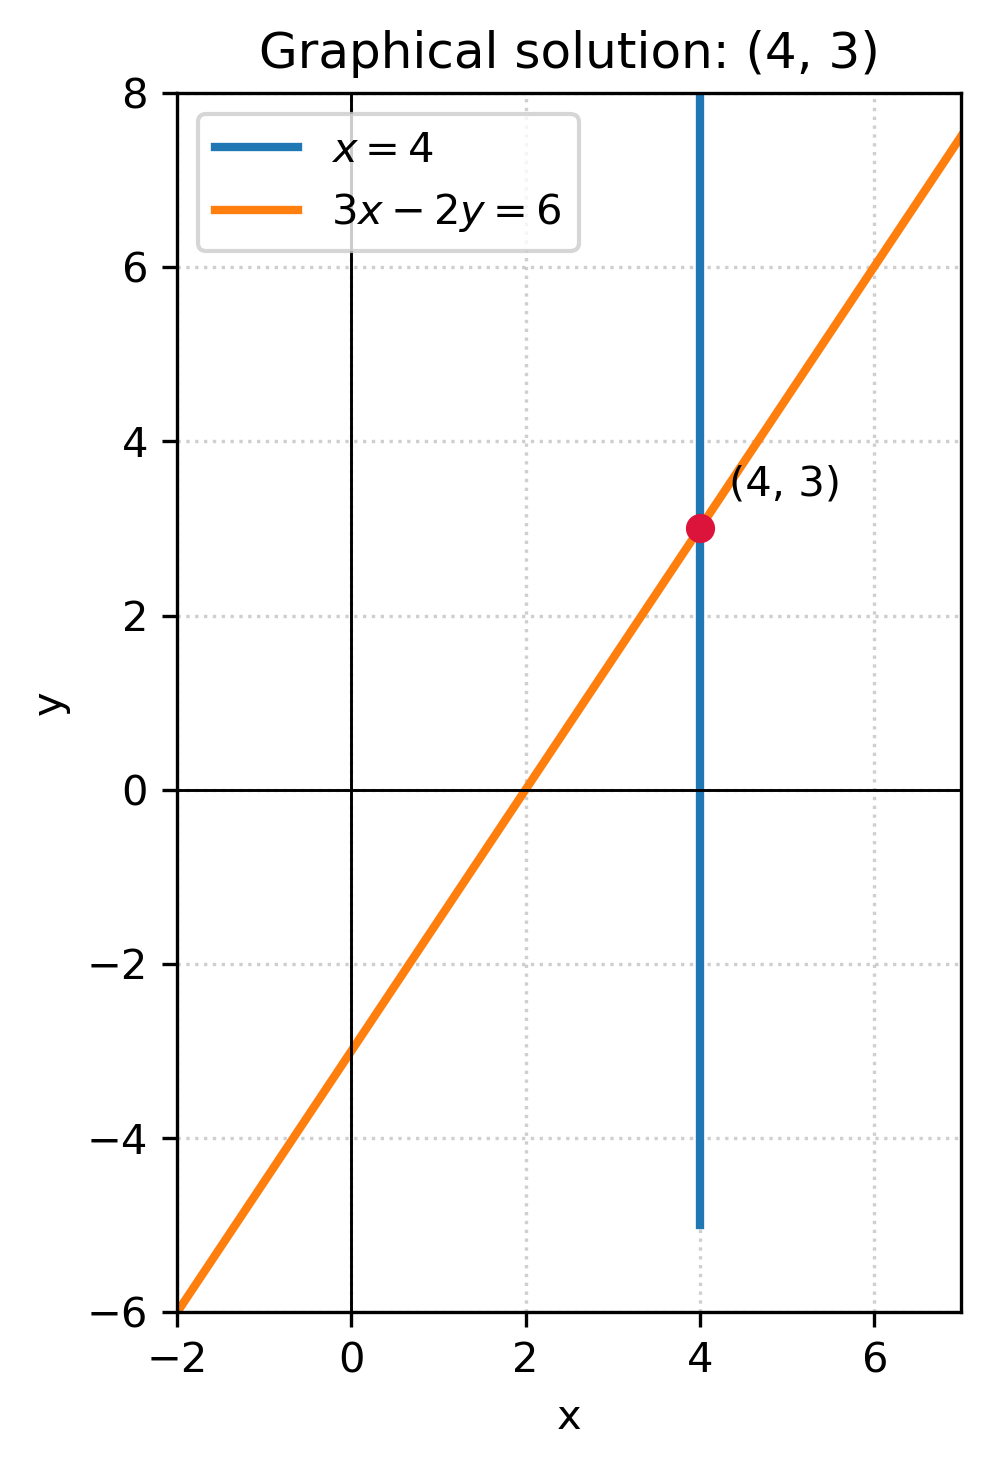
\includegraphics[width=0.27\linewidth]{figs/5.1.30.png}
\caption{Graphs of the two equations and their intersection.}
\label{fig:q30}
\end{figure}
\end{list}
\vspace{1.2em}
\begin{list}{}{\setlength{\leftmargin}{1.15cm}\setlength{\labelwidth}{1.0cm}\setlength{\labelsep}{0.15cm}\setlength{\itemindent}{0pt}\setlength{\listparindent}{0pt}\setlength{\parsep}{0pt}\setlength{\topsep}{0pt}}\setlist[enumerate]{leftmargin=0.7cm}
\item[5.1.31] A window measures $156$ cm by $216$ cm. It is to be covered with the largest possible equal square tiles. Find the side of each square and the number of squares.

\vspace{0.7em}\par\noindent\textbf{Solution:} The greatest common divisor of 156 and 216 is 12. Each square has side 12 cm, and the number of squares is $\frac{156}{12}\times\frac{216}{12}=13\times18=234$.

\begin{lstlisting}[frame=single, basicstyle=\rmfamily, escapeinside={(*@}{@*)}]
(*@\makebox[\dimexpr\linewidth-2\fboxsep-2\fboxrule\relax][c]{codes/5.1.31.py}@*)
\end{lstlisting}
\begin{figure}[H]
\centering
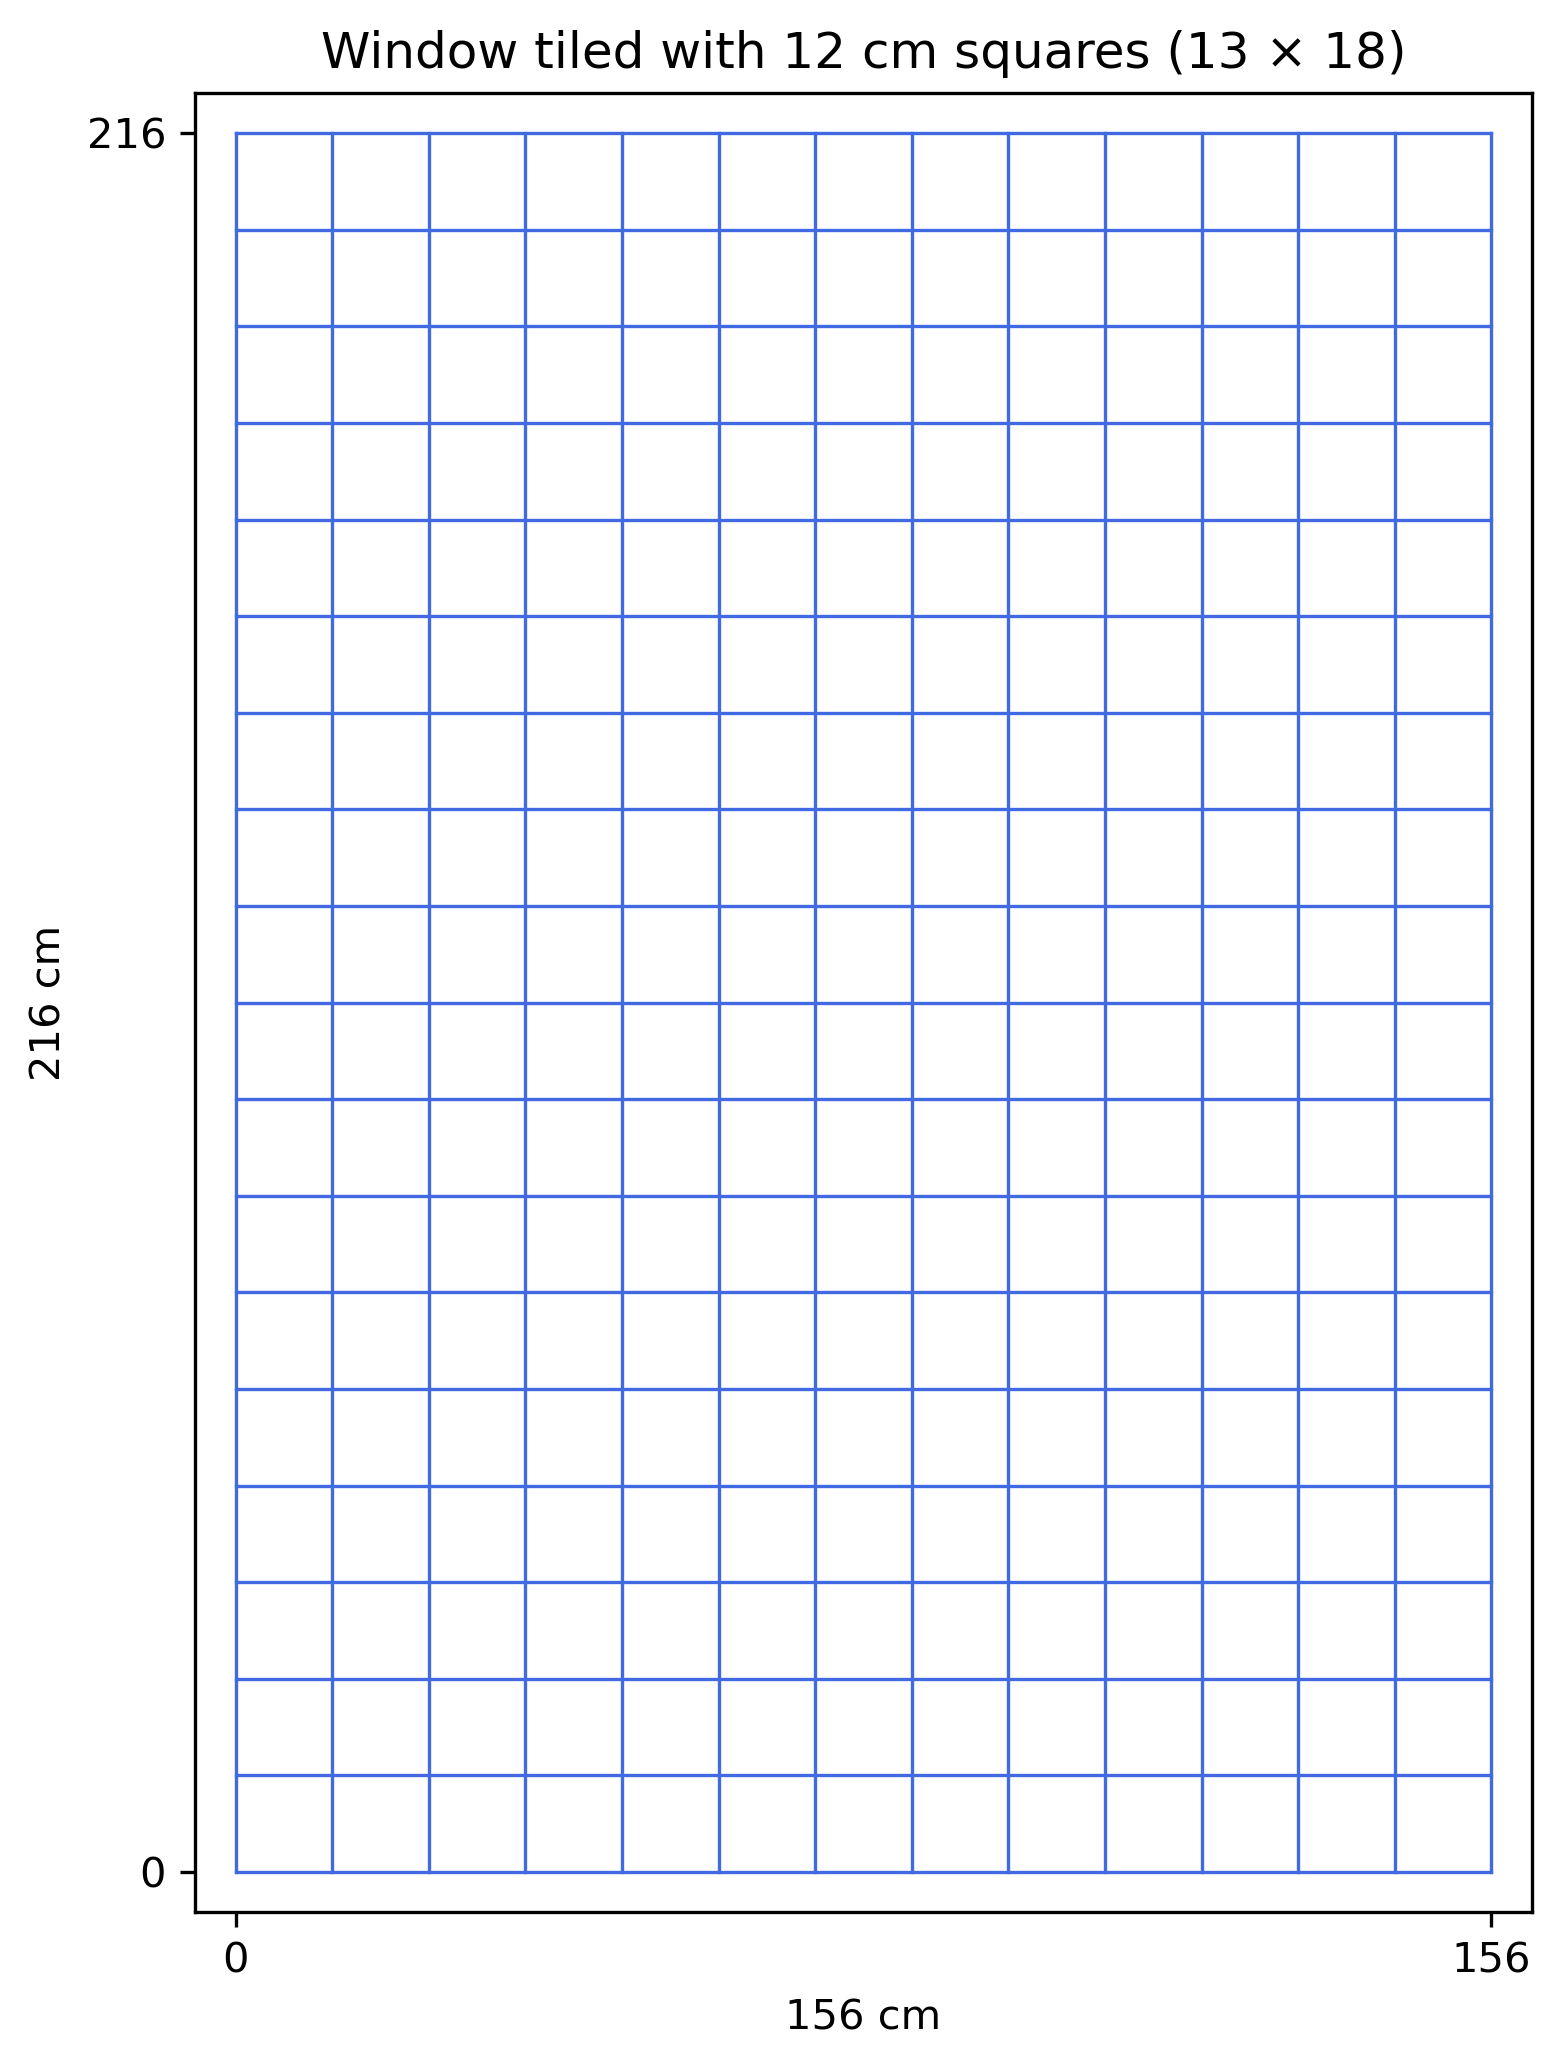
\includegraphics[width=0.30\linewidth]{figs/5.1.31.png}
\caption{Window divided into the largest equal square tiles.}
\label{fig:q31}
\end{figure}
\end{list}
\vspace{1.2em}
\begin{list}{}{\setlength{\leftmargin}{1.15cm}\setlength{\labelwidth}{1.0cm}\setlength{\labelsep}{0.15cm}\setlength{\itemindent}{0pt}\setlength{\listparindent}{0pt}\setlength{\parsep}{0pt}\setlength{\topsep}{0pt}}\setlist[enumerate]{leftmargin=0.7cm}
\item[5.1.35] Two tangents $PQ$ and $PR$ are drawn from $P$ to a circle with centre $O$ and radius 5 cm. The line $OP$ meets the circle at $C$, where another tangent $AB$ is drawn. If $OP=13$ cm, find $AB$ and $PA$.

\vspace{0.7em}\par\noindent\textbf{Solution:} Take $O=(0,0)$, $P=(13,0)$ and $C=(5,0)$. The tangent points from $P$ have coordinates $(25/13,\pm60/13)$. Their tangent lines meet $x=5$ at $A,B=(5,\pm10/3)$. Therefore $AB=20/3$ cm and $PA=26/3$ cm.

\begin{lstlisting}[frame=single, basicstyle=\rmfamily, escapeinside={(*@}{@*)}]
(*@\makebox[\dimexpr\linewidth-2\fboxsep-2\fboxrule\relax][c]{codes/5.1.35.py}@*)
\end{lstlisting}
\begin{figure}[H]
\centering
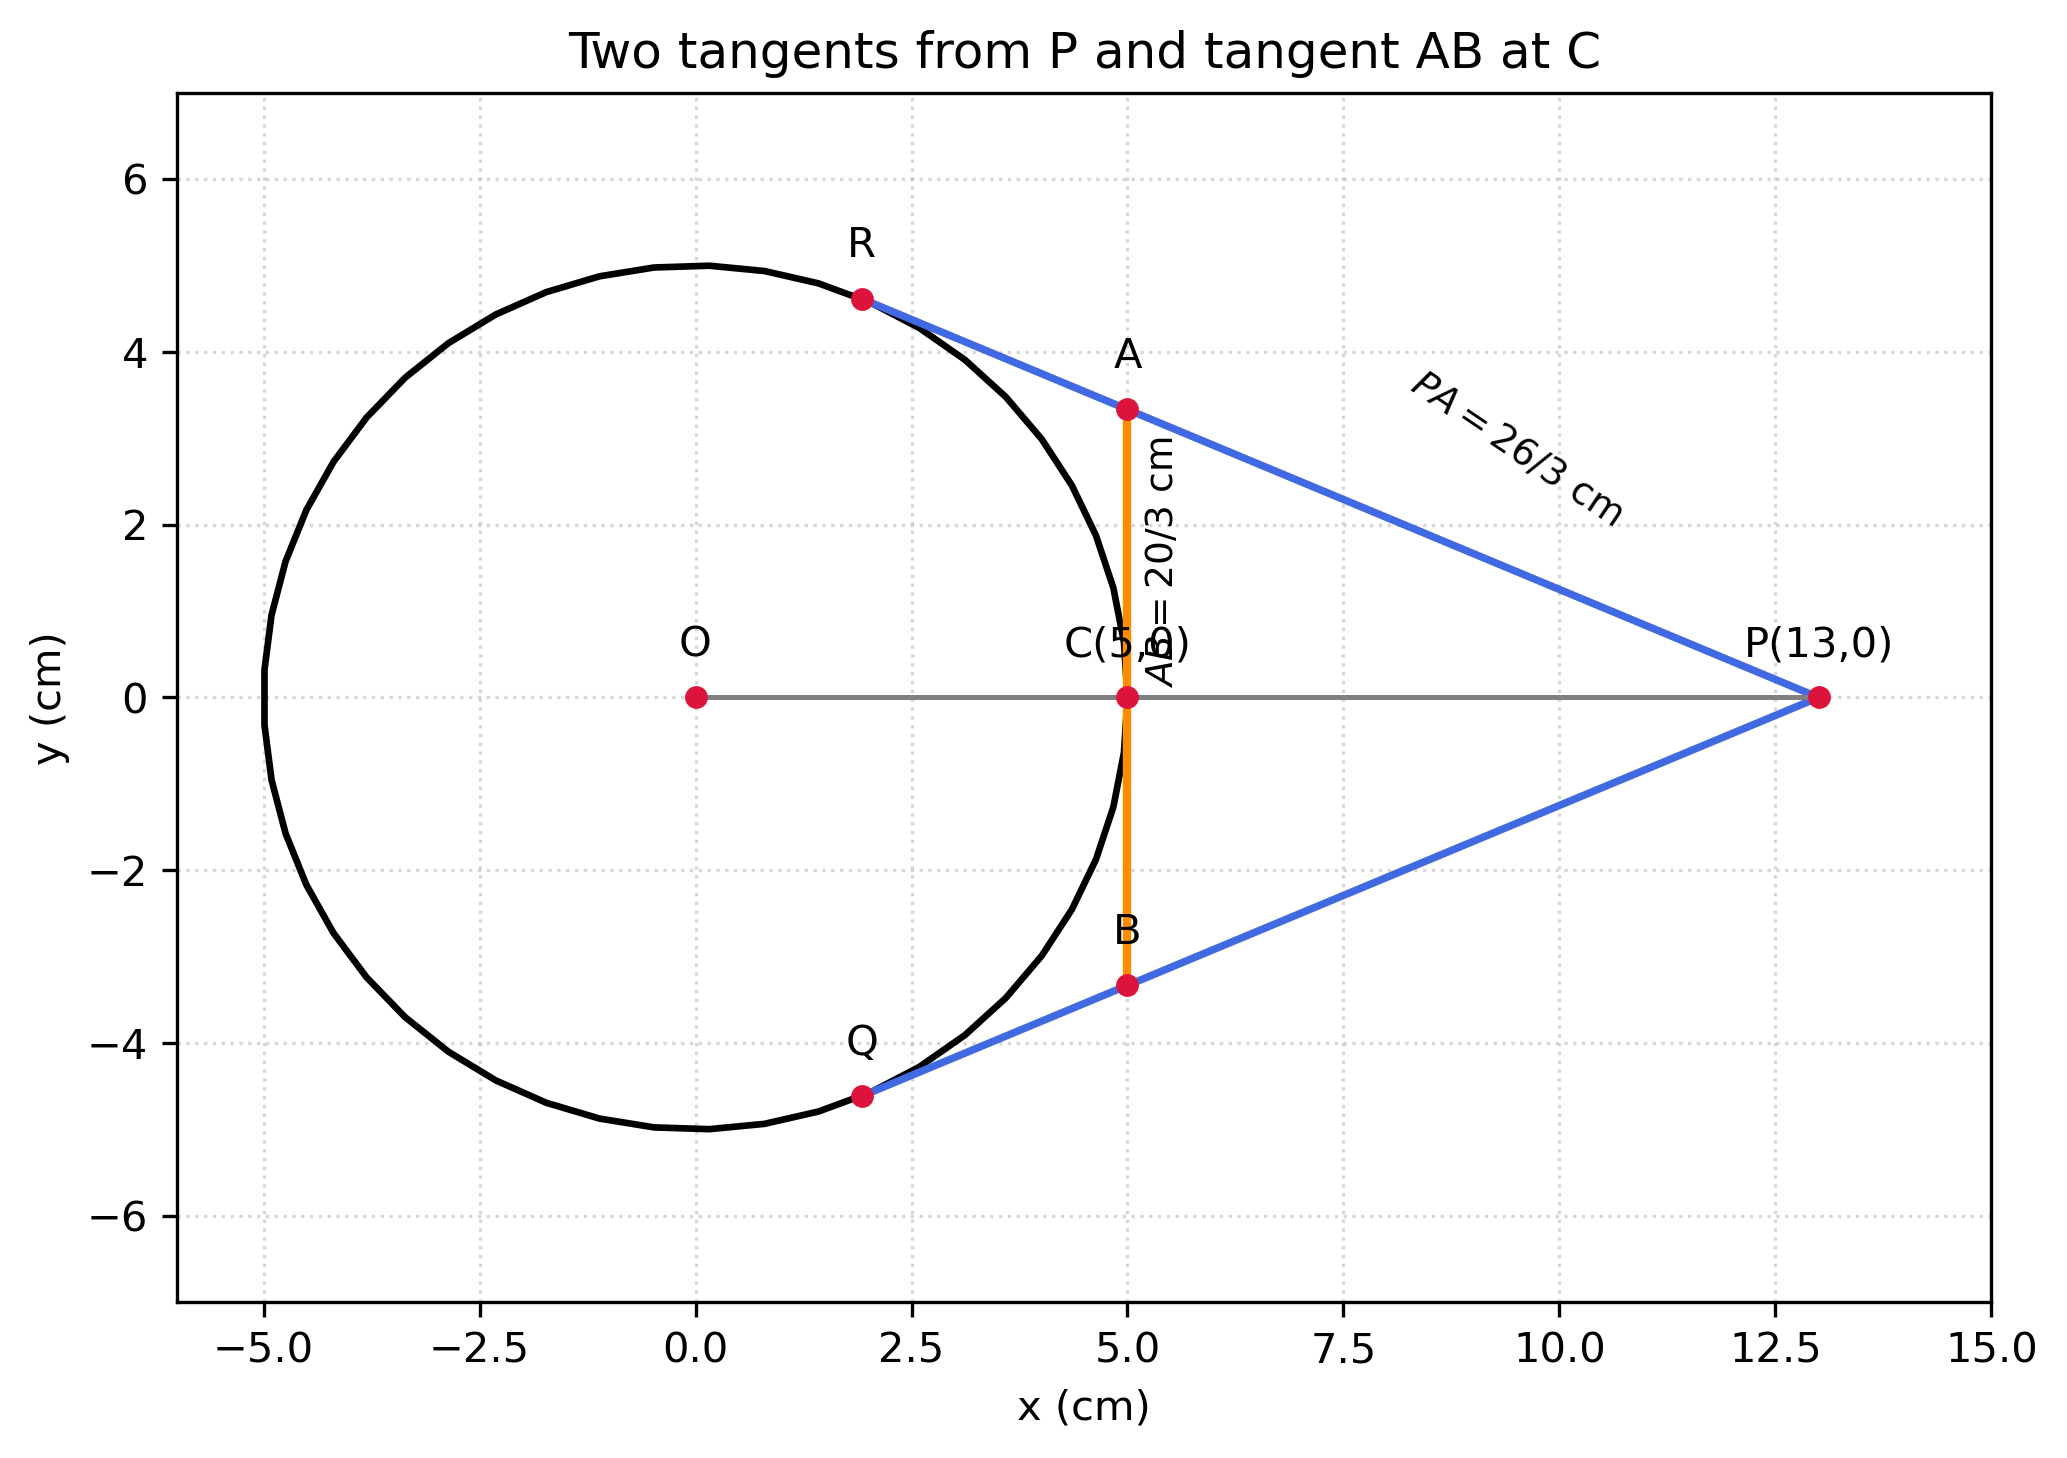
\includegraphics[width=0.53\linewidth]{figs/5.1.35.png}
\caption{Tangents from $P$ and the tangent $AB$ at $C$.}
\label{fig:q35}
\end{figure}
\end{list}
\vspace{1.2em}
\begin{list}{}{\setlength{\leftmargin}{1.15cm}\setlength{\labelwidth}{1.0cm}\setlength{\labelsep}{0.15cm}\setlength{\itemindent}{0pt}\setlength{\listparindent}{0pt}\setlength{\parsep}{0pt}\setlength{\topsep}{0pt}}\setlist[enumerate]{leftmargin=0.7cm}
\item[5.1.36] A railway bridge arch is modelled by $p(x)=-0.0025x^2-0.025x+136$. Plot the arch and mark its vertex $A$ and its endpoints $P,Q$ on the riverbed.

\vspace{0.7em}\par\noindent\textbf{Solution:} The vertex is $A=(-5,136.0625)$. The intercepts are $x=-5\pm5\sqrt{2177}$, so the span is $10\sqrt{2177}\approx467.02$ m.

\begin{lstlisting}[frame=single, basicstyle=\rmfamily, escapeinside={(*@}{@*)}]
(*@\makebox[\dimexpr\linewidth-2\fboxsep-2\fboxrule\relax][c]{codes/5.1.36.py}@*)
\end{lstlisting}
\begin{figure}[H]
\centering
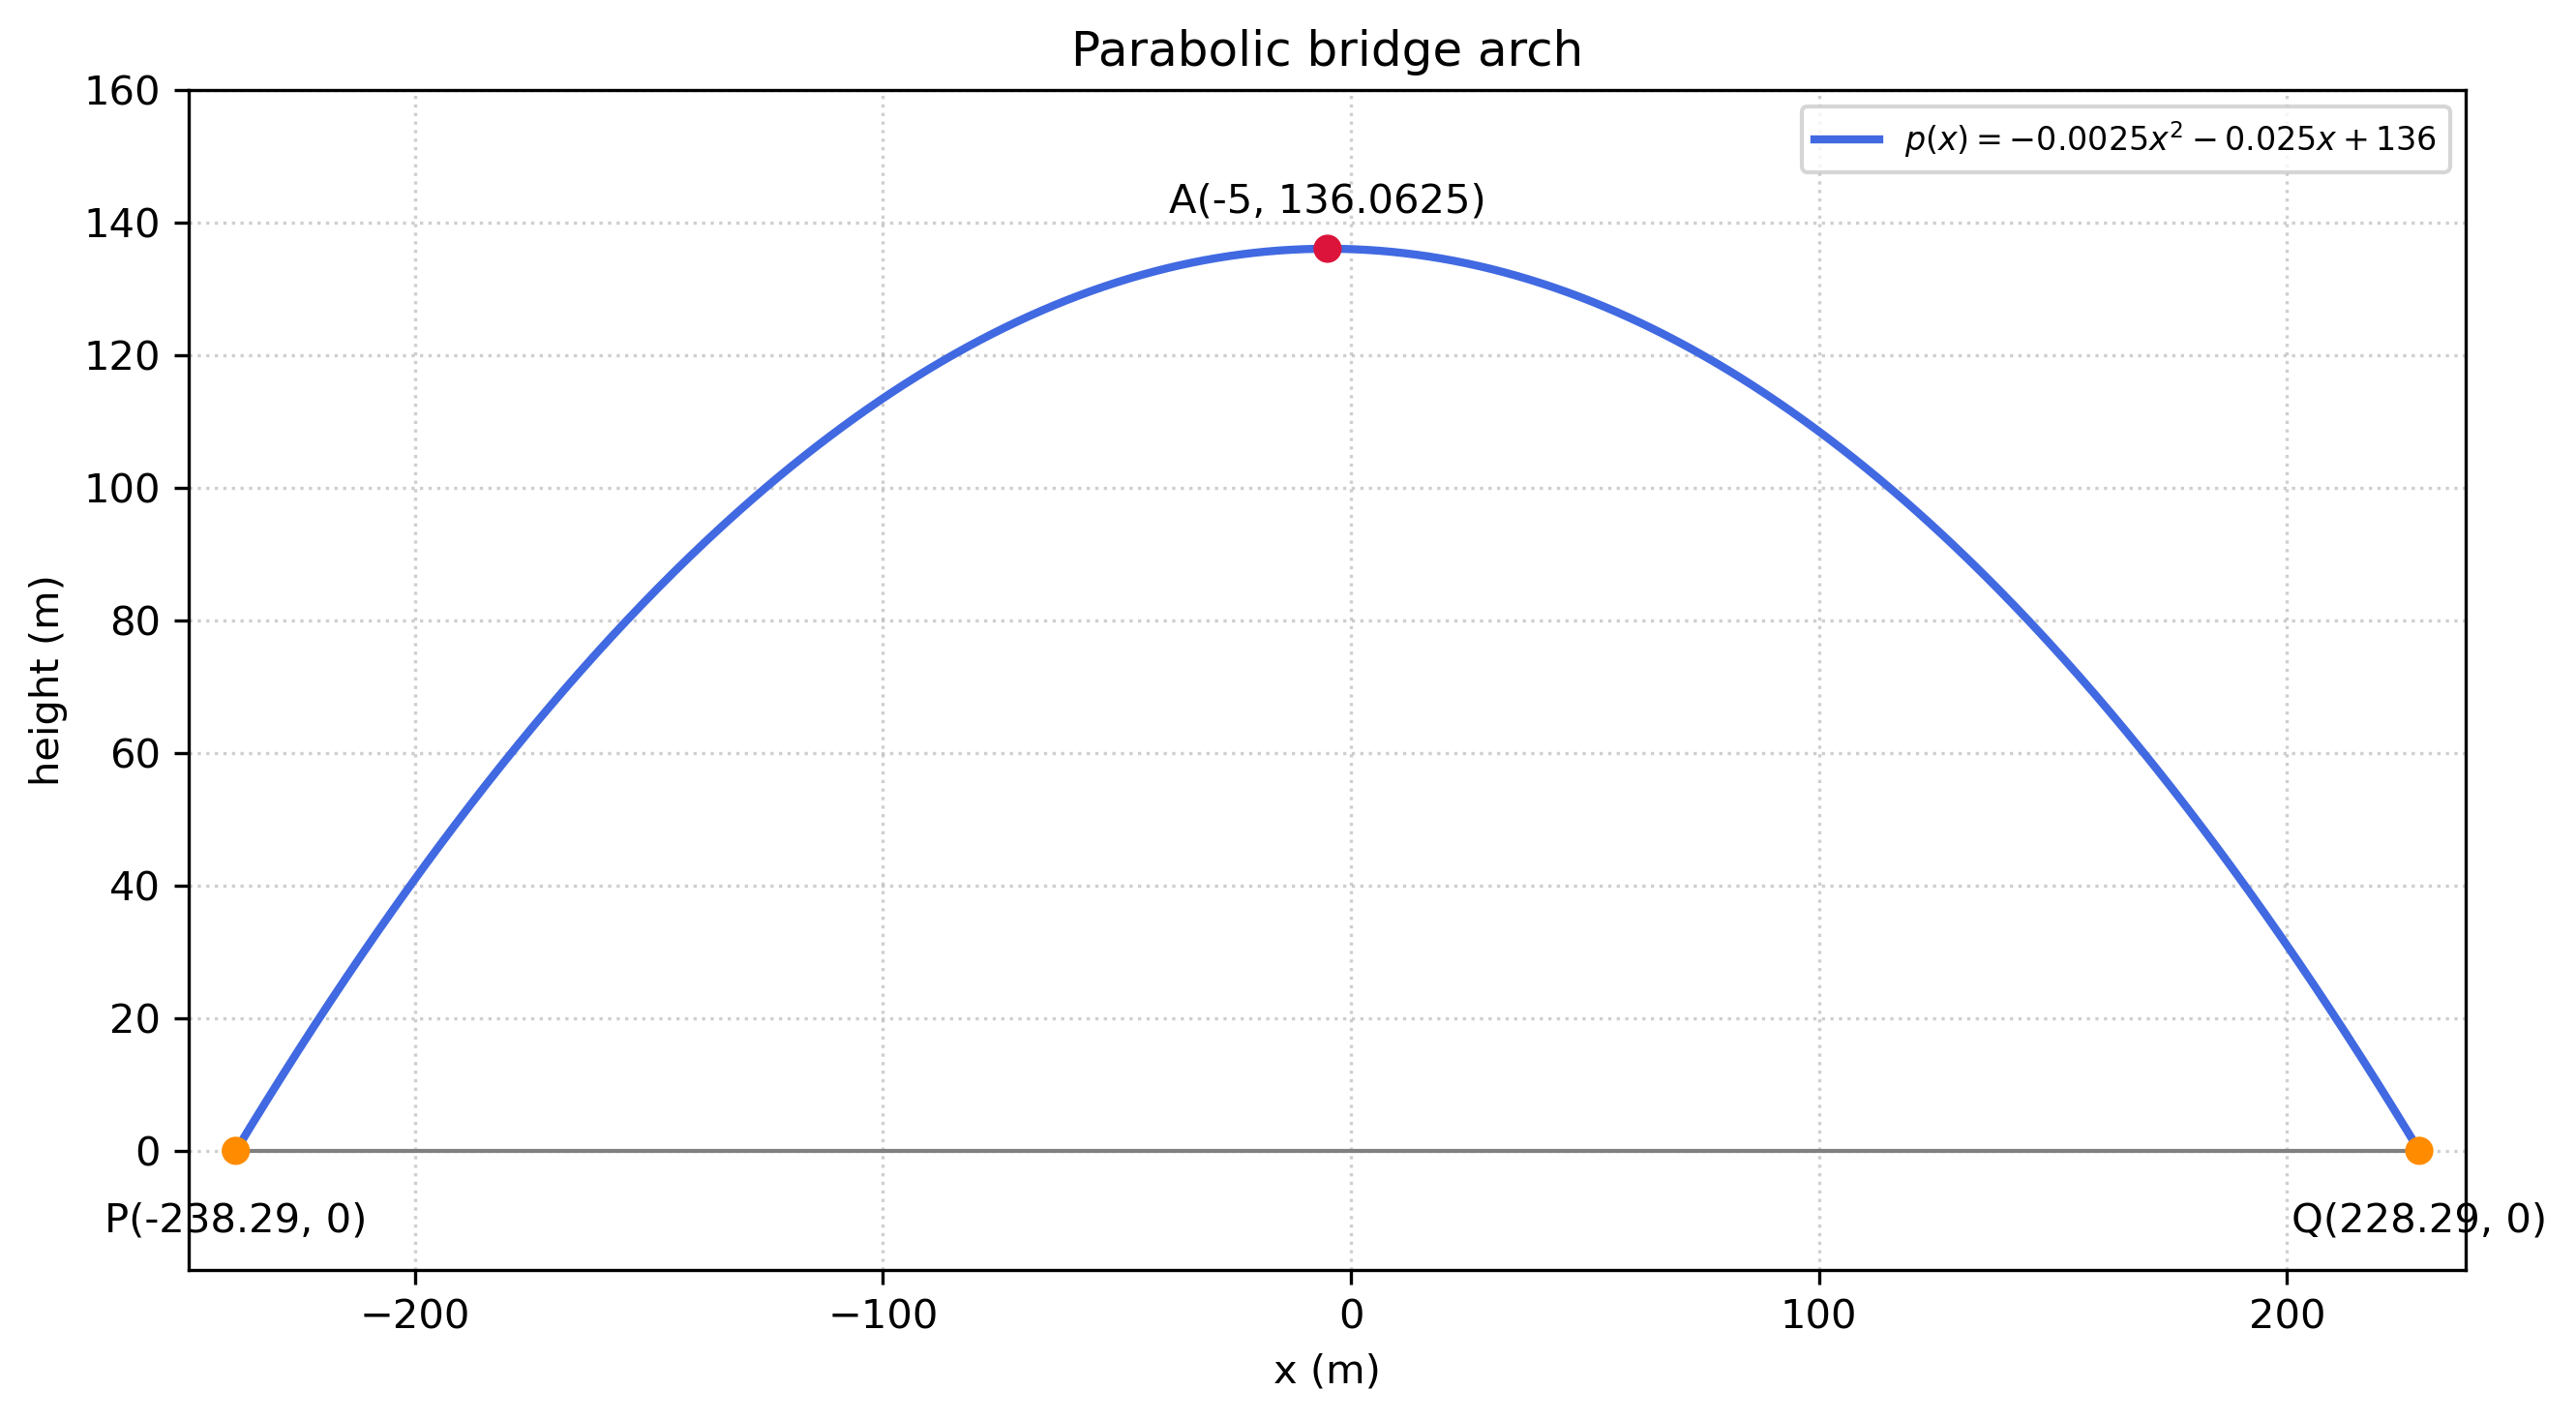
\includegraphics[width=0.44\linewidth]{figs/5.1.36.png}
\caption{Parabolic arch with vertex and riverbed endpoints marked.}
\label{fig:q36}
\end{figure}
\end{list}
\end{list}
\end{document}
